 %%%%%%%%%%%%%%%%%%%%%%%%%
 %%%%%%%%%%%%%%%%%%%%%%%%%
%%%Handouts for students to write on for entire semester
 %%%%%%%%%%%%%%%%%%%%%%%%%
 %%%%%%%%%%%%%%%%%%%%%%%%%

\documentclass[10pt,handout]{beamer} 
 
\usepackage{header100}
\usepackage{header_maps}

\setbeamertemplate{headline}{ %no ToC in headline -- too many chapters
%  \begin{beamercolorbox}[colsep=1.5pt]{upper separation line head}
%  \end{beamercolorbox}
}

\usepackage{pgfpages}
\pgfpagesuselayout{4 on 1}[letterpaper,border shrink=1mm,landscape,]
 %several slides per page, sized for printing


%https://tex.stackexchange.com/questions/75393/pgfpages-outer-border-instead-of-border-shrink
\newlength{\pageborder}
\setlength{\pageborder}{5mm}
\newlength{\pageborderBCOR}
\setlength{\pageborderBCOR}{10mm}
\pgfpagesphysicalpageoptions{
	   %border code=\pgfusepath{stroke}
	   }

\pgfpageslogicalpageoptions{1}{
          border code=\pgfusepath{stroke}
        , resized height=\dimexpr.5\pgfphysicalheight-\pageborder-.5\pageborderBCOR
        , resized width=\dimexpr.5\pgfphysicalwidth-\pageborder-.5\pageborderBCOR
        , center = \pgfpoint{.25\pgfphysicalwidth+\pageborder}%
                                  {.75\pgfphysicalheight-.5\pageborder-.75\pageborderBCOR}
}
\pgfpageslogicalpageoptions{2}{
          border code=\pgfusepath{stroke}
        , resized height=\dimexpr.5\pgfphysicalheight-\pageborder-.5\pageborderBCOR
        , resized width=\dimexpr.5\pgfphysicalwidth-\pageborder-.5\pageborderBCOR
        , center = \pgfpoint{.75\pgfphysicalwidth-\pageborder}%
                                  {.75\pgfphysicalheight-.5\pageborder-.75\pageborderBCOR}
}
\pgfpageslogicalpageoptions{3}{
          border code=\pgfusepath{stroke}
        , resized height=\dimexpr.5\pgfphysicalheight-\pageborder-.5\pageborderBCOR
        , resized width=\dimexpr.5\pgfphysicalwidth-\pageborder-.5\pageborderBCOR
        , center = \pgfpoint{.25\pgfphysicalwidth+\pageborder}%
                                  {.25\pgfphysicalheight+.5\pageborder-.25\pageborderBCOR}
}
\pgfpageslogicalpageoptions{4}{
          border code=\pgfusepath{stroke}
        , resized height=\dimexpr.5\pgfphysicalheight-\pageborder-.5\pageborderBCOR
        , resized width=\dimexpr.5\pgfphysicalwidth-\pageborder-.5\pageborderBCOR
        , center = \pgfpoint{.75\pgfphysicalwidth-\pageborder}%
                                  {.25\pgfphysicalheight+.5\pageborder-.25\pageborderBCOR}
}



\begin{document}
 %%%%%%%%%%%%%%%%%%%%%%%%%
 %%%%%%%%%%%%%%%%%%%%%%%%%
 %%%%%%%%%%%%%%%%%%%%%%%%
% 
%%chapter 1
\foreach \n in {1,...,6}{
\input{sections/1_\n.tex}
}
%optional sections
%% Copyright 2021 Joel Feldman, Andrew Rechnitzer and Elyse Yeager, except where noted.
% This work is licensed under a Creative Commons Attribution-NonCommercial-ShareAlike 4.0 International License.
% https://creativecommons.org/licenses/by-nc-sa/4.0/


%------------------------------------------------------
\section[1.8 Formal Limits at Infinity]{1.8 (Optional) Making Infinite Limits a Little More Formal}

 \begin{frame}{Table of Contents}
\begin{center}1.8 (Optional) Making Infinite Limits a Little More Formal\end{center}
\mapofcontentsA{}
 \end{frame}
%------------------------------------------------------
\note{One conceptual hurdle I've noticed with students is that the epsilon-delta definitions just have a lot of variables, and it's tough to remember which is which. I've had success in the past with the model below, I think because it disambiguates the parameters. Rather than an abstract list of variable names, it gives us a story with pieces that are easy to distinguish. ``The amount you put in the can," ``the amount your boss wants you to put in a can,"  ``the time you've been working," and ``the error in your can weight" are easier to keep straight then ``$f(x)$", ``$L$",  ``$x$," and ``$\epsilon$".
\\[1em]

Because limits at infinity have fewer moving parts (notably: you only have to worry about one ``side), I like to teach 1.8 \textit{before} 1.7.}
%------------------------------------------------------

\begin{frame}[t]
You work at a salmon cannery, putting salmon into cans. Each can is supposed to contain the amount of salmon shown on the label, but some error is allowable. As you work longer, and get more experience, the amount of error you are allowed to have gets smaller.
\vfill

\begin{tikzpicture}
%shrinking error margins
\onslide<2-4|handout:0>{
	\ycoord[C1]{1}{250}
	\ycoord[C1]{3}{750}}
\onslide<3-4|handout:0>{
	\draw[help lines] (0,1)--(9,1) (0,3)--(9,3);}
\onslide<4-4|handout:0>{
	\fill[W5] (1.1,1) rectangle (9.3,3)  (1,-.2) rectangle (1.4,-.7);}

\onslide<5-7|handout:0>{
	\ycoord[C1]{1.5}{375}
	\ycoord[C1]{2.5}{625}}
\onslide<6-7|handout:0>{
	\draw[help lines] (0,1.5)--(9,1.5) (0,2.5)--(9,2.5);}
\onslide<7-7|handout:0>{
	\fill[W5] (5.1,1.5) rectangle (9.3,2.5) (4.7,-.2) rectangle (5.3,-.7);
}


\onslide<8-10|handout:0>{
	\ycoord[C1]{1.6}{400}
	\ycoord[C1]{2.4}{600}}
\onslide<9-10|handout:0>{
	\draw[help lines] (0,1.6)--(9,1.6) (0,2.4)--(9,2.4);}
\onslide<10|handout:0>{
	\fill[W5] (7.1,1.6) rectangle (9.3,2.4) (7.2,-.2) rectangle (7.8,-.7);
}


%graph
\myaxis{t}{0}{9.25}{}{0}{3.5}
\ycoord{2}{500}
\foreach \x in {0,...,8}{
	\POWER{1.2}{-\x}{\a}
	\POWER{1.6}{-\x}{\b}
	\draw(\x+1,2+\a)node[]{
\includegraphics[width=2.5mm]{Clipart/can}};
	\draw(\x+0.5,2+\b)node[]{
\includegraphics[width=2.5mm]{Clipart/can}};
	\draw(\x+.25,2-\a)node[]{
\includegraphics[width=2.5mm]{Clipart/can}};
	\draw(\x+0.75,2-\b)node[]{
\includegraphics[width=2.5mm]{Clipart/can}};	
	}
\foreach \x in {1,...,36}{
	\xcoord{\x/4}{}}
\foreach \x in {5,10,...,35}{
	\xcoord{\x/4}{\x}}
\end{tikzpicture}
\index{
\includegraphics[height=5mm]{Clipart/can} ~\href{https://thenounproject.com/term/tuna-can/1453898/}{tuna can} by \href{https://thenounproject.com/throwawayicons/}{throwaway icons} is licensed under \CCBYthree}
\vfill

\color{C1}
\only<2-4>{Was there a time after which your error always \textit{less than} \alert{250} g?}
\only<5-7|handout:0>{Was there a time after which your error always \textit{less than} \alert{125} g?}
\only<8-10|handout:0>{Was there a time after which your error always \textit{less than} \alert{100} g?}
\note<3>{Emphasize: we don't really care exactly what that time was, we only need to know that it exists}
\note<6>{Good to point out that earlier, you were sometimes \textit{but not always} within the specified error tolerance. Non-monotone convergence is a common conceptual sticking point.}
\end{frame}

%------------------------------------------------------

\begin{frame}[t]
\AnswerSpace
\foreach \x in {1,...,5}{
	\MULTIPLY{\x}{2}{\A}
	\SUBTRACT{\A}{1}{\Q}
	\only<\Q>{\QuestionBar{\x}{5}\AnswerYes}
	\only<\A>{\AnswerBar{\x}{5}}
	}

Suppose the amount of salmon that is supposed to be in a can is 500 g. The amount of salmon you put into a can at time $x$ is $500+\frac6x$. 

\vfill

You need to reassure your boss that, after some time, your error is never more than \alert{\only<1-2>{3}\only<3-4|handout:0>{2}\only<5-6|handout:0>{1}\only<7-8|handout:0>{$\frac{1}{1000}$}\only<9-10|handout:0>{$\epsilon$} g}. Find such a time.
\vfill


\begin{tikzpicture}[xscale=0.75]%space to write on RHS
\myaxis{x}{0}{9.25}{}{0}{3.2}
\ycoord{1.5}{500}
\draw[dashed] (0,1.5)--(9,1.5);
\draw[double] (-.1,.5)--(.1,.5);
\draw[thick] plot[domain=0.5:9,smooth,samples=50]({\x},{1.25+1/(.2*\x+0.4)})node[above left]{$f(x)=500+\frac{6}{x}$};

	\color{W1}
	\onslide<2|handout:0>{\draw (0,2.5)-|(2,0);
		\ycoord{2.5}{503}
		\xcoord{2}{2}
	}
	\onslide<4|handout:0>{\draw (0,2.25)-|(3,0);
		\ycoord{2.25}{502}
		\xcoord{3}{3}
	}
	\onslide<6|handout:0>{\draw (0,1.875)-|(6,0);
		\ycoord{1.875}{501}
		\xcoord{6}{6}
	}

\end{tikzpicture}

\answer{\color{answercolor}
\foreach \s/\x/\y in {1/2/3,3/3/2,5/6/1,7/6000/\frac{1}{1000},9/\frac{6}{\epsilon}/\epsilon}{
	\ADD{\s}{1}{\ss}
\only<\s-\ss>{When $x > \onslide<\ss>{\x}$\quad then $|f(x)-500|< \y $.}
}}

\onslide<10>{No matter how exacting your boss is, if they give you a non-zero error allowance, you can \textit{always} schedule a time after which you will meet their standards.}
\end{frame}
%------------------------------------------------------
\begin{frame}[t]
\begin{block}{Definition~\eref{text}{def_1_8_1} (a)}
  Let $f$ be a function defined on the whole real line. We say that
\begin{quote}
  the limit as $x$ approaches $\infty$ of $f(x)$ is $L$
\end{quote}\\
and write
\begin{align*}
  \lim_{x \to \infty} f(x) &= L
\end{align*}
if and only if for every $\epsilon>0$ there exists $M \in \mathbb{R}$ so that
$|f(x)-L| < \epsilon$ whenever $x>M$.

Similarly we write
\begin{align*}
  \lim_{x \to -\infty} f(x) &= K
\end{align*}
if and only if for every $\epsilon>0$ there exists $N \in \mathbb{R}$ so that
$|f(x)-K| < \epsilon$ whenever $x<N$.


\end{block}
\end{frame}

%------------------------------------------------------

\begin{frame}
\begin{tabular}{p{0.5\textwidth} p{0.5\textwidth}}
\alert<1>{  Let $f$ be a function defined on the whole real line. } & \color{C1} $f(x)$:  actual can weights\\ \pause
%
\raggedright \alert<2>{ We say that
``the limit as $x$ approaches $\infty$ of $f(x)$ is $L$"
and write
\begin{align*}
  \lim_{x \to \infty} f(x) &= L
\end{align*}}& 
\color{C1} $L$: weight on the label that you want to match\\\pause
%
\alert<3>{if and only if for every $\epsilon>0$}
&
\color{C1} $\epsilon$: amount of allowable error
\\\pause
%
\raggedright\alert<4>{there exists $M \in \mathbb{R}$ so that
${|f(x)-L| < \epsilon}$ whenever $x>M$.}
&
\color{C1} $M$: time after which your weights are always off by less than $\epsilon$\\[1mm]
&\color{C1}$|f(x)-L|$: error  (difference between actual amount and label)
\end{tabular}\pause


\end{frame}

%------------------------------------------------------

\begin{frame}
\begin{tikzpicture}
\myaxis{x}{0}{8}{y}{0}{2}
\draw[thick] plot[domain=0:8,samples=100,smooth](\x,{1+0.75*sin(\x*5 r)*(1-\x/8.5)})node[right]{$y=f(x)$};
\onslide<2->{\ycoord{1}{L}}
\onslide<3-|handout:0>{
\color{W1}
\ycoord[above left]{1.2}{L+\epsilon}
\ycoord[below left]{0.8}{L-\epsilon}
\draw[dashed] (.2,1.2)--(8,1.2) (.2,0.8)--(8,0.8);
\onslide<4-|handout:0>{\xcoord{6.1}{M}}
}
\end{tikzpicture}
\vfill
\alert<1|handout:0>{  Let $f$ be a function defined on the whole real line. } \pause
 \alert<2|handout:0>{ We say that
``the limit as $x$ approaches $\infty$ of $f(x)$ is $L$"
and write
\begin{align*}
  \lim_{x \to \infty} f(x) &= L
\end{align*}}\pause
\alert<3|handout:0>{if and only if for every $\epsilon>0$} \pause
\alert<4|handout:0>{there exists $M \in \mathbb{R}$ so that
${|f(x)-L| < \epsilon}$ whenever $x>M$.}
\end{frame}

%------------------------------------------------------

\begin{frame}[t]
 \note<1>{For easy questions, students may wonder what the use of the definition is. Point out in later examples that it clears up ambiguity when the function is less obvious.}

\note<2>{Two things to note. One, that we have to find $M$, and that part is separate from the actual proof we write down. Two, we get to assume $x$ is large (so in this case, positive) because we only care about values larger than $M$. Remind students our cannery boss didn't care about our initial novice imprecision.}

\begin{block}{Definition~\eref{text}{def_1_8_1} (a)}
  Let $f$ be a function defined on the whole real line. We say that
$  \dlimx{\infty} f(x) = L$
if and only if for every $\epsilon>0$ there exists $M \in \mathbb{R}$ so that
$|f(x)-L| < \epsilon$ whenever $x>M$.
\end{block}
\color{C1}
\begin{QuestionSet}
\SetQuestion{%Q1
\AnswerYes
 Prove, using Definition \eref{text}{def_1_8_1}, that $\dlimx{\infty}\left[\frac2x+1\right] = 1$.}
\SetAnswer{\small
 Prove, using Definition \eref{text}{def_1_8_1}, that $\dlimx{\infty}\left[\frac2x+1\right] = 1$.\\
 \color{answercolor}
\begin{multicols}{2}Let $\epsilon$ be any positive constant. We need to find $M$ such that, for $x>M$:
\begin{align*}
\left|f(x)-L\right|&<\epsilon\\
\left|\left(\frac2x+1\right)-1\right|&<\epsilon\\
\left|\frac2x\right|&<\epsilon
\intertext{It suffices to find a positive $M$. Then $x$ is positive too.}
\frac2x&<\epsilon\\
x&>\frac2{\epsilon}
\end{align*}
So, we choose $M = \frac2{\epsilon}$. Now we can go through the definition.
\end{multicols}
}
\SetAnswer{
 Prove, using Definition \eref{text}{def_1_8_1}, that $\dlimx{\infty}\left[\frac2x+1\right] = 1$.\\\vfill
 \color{answercolor}
\textbf{Proof: }
Let $f(x) = \frac2x+1$. For any $\epsilon>0$, let $M = \frac{2}{\epsilon}$. Then for any $x>M$:
\begin{align*}
|f(x)-1|&=\left| \left(\frac2x+1\right)-1\right| = \left| \frac2x\right|=\frac2x\\
&<\frac2M = \frac{2}{\frac{2}{\epsilon}}=\epsilon
\end{align*}
Therefore $\dlimx{\infty}\left[\frac2x+1\right]=1$.\qed
}


%Q2
\SetQuestion{
\AnswerYes
  Prove, using Definition \eref{text}{def_1_8_1}, that  $\dlimx{\infty}\left[ 5e^{-x} \right]=0$}
\SetAnswer{
 Prove, using Definition \eref{text}{def_1_8_1}, that  $\dlimx{\infty}\left[ 5e^{-x} \right]=0$

 \color{answercolor}
 First, we need to find which $M$ goes with $\epsilon.$
 \begin{align*}
 |f(x)-L|&=\left| 5e^{-x}-0\right| = 5e^{-x}=
 \frac{5}{e^x}<\epsilon\\
 e^x &>\frac{5}{\epsilon}\\
 x&>\log_e\left(\frac5\epsilon\right)
 \end{align*}
 So, in our proof, we should use $M=\log_e\left(\frac5\epsilon\right)$
 }
 \SetAnswer{
 Prove, using Definition \eref{text}{def_1_8_1}, that  $\dlimx{\infty}\left[ 5e^{-x} \right]=0$

 \color{answercolor}
\textbf{Proof: } Set $f(x) = 5e^{-x}$. For any $\epsilon>0$, let $M = \log_e\left(\frac5\epsilon\right)$. Then for all $x$ that are greater than $M$:
\begin{align*}
\left| f(x)-0\right|&=\left| 5e^{-x}\right| = \frac{5}{e^x}\\
&<\frac{5}{e^M} = \frac{5}{e^{\log_e\left(\frac5e\right)}} = \frac{5}{\frac5\epsilon} = \epsilon
\end{align*}
Therefore, $\dlimx{\infty}[5e^{-x}]=0$. \qed
 }
 


%Q3
\SetQuestion{
\AnswerYes
\NowYou Prove, using Definition \eref{text}{def_1_8_1}, that   $\dlimx{\infty}\left[ \frac{\sin x}{x} \right]=0$
}
\SetAnswer{
 Prove, using Definition \eref{text}{def_1_8_1}, that   $\dlimx{\infty}\left[ \frac{\sin x}{x} \right]=0$

 \color{answercolor}
 \begin{multicols}{2}
 First, we find $M$ for an arbitrary $\epsilon$. We want
\[
|f(x) - 0|=\left|\frac{\sin x}{x}\right| < \epsilon
\]
We need to find values of $x$ that are large enough for this to be true, but we don't have to find the values of $x$ that make equality hold. (Think about the first canning example where we didn't even have numbers.) So, we simplify things by noting $|\sin x |<1$ for all $x$. For $x>0$,

 \begin{align*}
\left|\frac{\sin x}{x} \right|<\left| \frac1x\right| = \frac1x&<\epsilon\\
x&>\frac1\epsilon
 \end{align*}
 So, we use $M = \frac1\epsilon$.
\end{multicols}
 }\SetAnswer{
 Prove, using Definition \eref{text}{def_1_8_1}, that   $\dlimx{\infty}\left[ \frac{\sin x}{x} \right]=0$

 \color{answercolor}
\textbf{ Proof: }
Let $f(x) = \frac{\sin x}{x}$. For any $\epsilon>0$, let $M = \frac1\epsilon$. Whenever $x>M$:
\begin{align*}
\left| f(x)-0\right|&=\left| \frac{\sin x}{x}\right|\leq \left| \frac1x\right| = \frac1x\\
&<\frac1M = \epsilon
\end{align*}
So $\dlimx{\infty}\frac{\sin x}{x} = 0$. \qed
 }


%Q4
\SetQuestion{
\AnswerYes
\NowYou  Prove, using Definition \eref{text}{def_1_8_1}, that  $\dlimx{\infty}\left[\frac{2x^2}{x^2+1}\right]=2$ }
\SetAnswer{
Prove, using Definition \eref{text}{def_1_8_1}, that  $\dlimx{\infty}\left[\frac{2x^2}{x^2+1}\right]=2$ 

 \color{answercolor}

First, we find $M$ based on $\epsilon$.
\begin{align*}
\epsilon & >|f(x) - 2|=\left| \frac{2x^2}{x^2+1} - 2\right| = \left| \frac{2x^2-2(x^2+1)}{x^2+1}\right| = \left| \frac{-2}{x^2+1} \right|
=\frac{2}{x^2+1}\\
x^2+1&>\frac2\epsilon \implies x^2>\frac2\epsilon - 1
\implies x>\sqrt{\frac2\epsilon - 1}=M
\end{align*}
(If $\epsilon>2$, we can take $M=0$.)
Note that the values of $x$ that make $x^2>\frac2\epsilon - 1$ true are $(-\infty,-a) \cup (a,\infty)$ for $a=\sqrt{\frac2\epsilon - 1}$. Since we only care about large $x$, we use the second interval. (See graph on next slide.)
}
\SetAnswer{
 Prove, using Definition \eref{text}{def_1_8_1}, that  $\dlimx{\infty}\left[\frac{2x^2}{x^2+1}\right]=2$ 
\begin{tikzpicture}
\color{black}
\myaxis{x}{3}{3}{y}{0}{3}
\draw[C1, thick] plot[domain=-3:3](\x,{\x*\x/3})node[right]{$y=x^2$};
\draw[dashed] (-3,4/3)--(3,4/3)node[right]{$\frac{2}{\epsilon}-1$};
\xcoord{2}{\sqrt{\frac{2}{\epsilon}-1}}
\xcoord{-2}{-\sqrt{\frac{2}{\epsilon}-1}}
\end{tikzpicture}\hfill
\parbox[b]{.3\textwidth}{\color{answercolor}\raggedright
	It \textbf{is true} that for all $x>\sqrt{\frac2\epsilon-1}$, $x^2>\frac2\epsilon-1$.\\[1em]
	It \textbf{is not true} that for all $x>-\sqrt{\frac2\epsilon-1}$, $x^2>\frac2\epsilon-1$.\\[2em]}	
}
\SetAnswer{
 Prove, using Definition \eref{text}{def_1_8_1}, that  $\dlimx{\infty}\left[\frac{2x^2}{x^2+1}\right]=2$ 

 \color{answercolor}
\textbf{ Proof: }: Let $f(x) = \frac{2x^2}{x^2+1}$. 
For any $2\ge\epsilon>0$, set $M = \sqrt{\frac2\epsilon - 1}$. 
                (For $\epsilon>2$, set $M=0$.)
                Then for any $x>M$:
\begin{align*}
|f(x) - 2| &=\left| \tfrac{2x^2}{x^2+1}-2 \right| = \left|\tfrac{-2}{x^2+1}\right| = \tfrac{2}{x^2+1}\\
&<\frac2{M^2+1} = \tfrac{2}{\left(\sqrt{\frac2\epsilon - 1}\right)^2+1} = \frac{2}{\frac2\epsilon-1+1}=\epsilon
\end{align*}
So $\dlimx{\infty}\left[\frac{2x^2}{x^2+1}\right]=2$.\qed
}


%Q5
\SetQuestion{
\AnswerYes
 Prove, using Definition \eref{text}{def_1_8_1}, that  $\dlimx{\infty} 5 = 5$
 }
\SetAnswer{
 Prove, using Definition \eref{text}{def_1_8_1}, that  $\dlimx{\infty} 5 = 5$

 \color{answercolor}
\textbf{ Proof: }: Let $f(x) = 5$, and let $M=1$. For any $\epsilon >0$, and for any $x>M$:
 \begin{align*}
 |f(x)-5| = 5-5 = 0 < \epsilon
 \end{align*}
 So, $\dlimx{\infty} 5 = 5$. \qed \\ \vfill
 Note: you actually could have chosen \textit{any} value for $M$.
 }


%Q6
\SetQuestion{
\AnswerYes
True or False? $\dlimx{\infty} \sin x = 0$
 }
\SetAnswer{
True or False? $\dlimx{\infty} \sin x = 0$

 \color{answercolor}
False.

Let $f(x)=\sin x$ and consider $\epsilon = \frac12$. Note that when $x=\frac{\pi}{2}+n\pi$ for any integer $n$, then $\sin x = \pm 1$, so
\[|f(x)-0| = |\pm 1|=1>\frac12\]
So there is \textit{no} point after which $f(x)$ is always within $\frac12$ of $0$. Therefore $\dlimx{\infty} \sin x \neq 0$.
 }
\SetAnswer{
True or False? $\dlimx{\infty} \sin x = 0$
\color{black}
\begin{tikzpicture}
\myaxis{x}{0}{8}{y}{1}{1}
\draw[C1, thick] plot[domain=0:8,smooth,samples=50](\x,{sin(3*\x r)})node[right]{$y=\sin x$};
\ycoord{.5}{0+\frac12}
\ycoord{-.5}{0-\frac12}
\draw[dashed] (.2,.5)--(8,.5) (.2,-.5)--(8,-.5);
\end{tikzpicture}
 }
 



 \end{QuestionSet}
\end{frame}

%------------------------------------------------------

\begin{frame}[t]{Useful General Principles}
When we showed $\dlimx{\infty}\left[\frac{\sin x}{x}\right]=0$, we chose $M$ using:
\[\left|\frac{\sin x}{x}\right|\le \left| \frac1x\right| = \frac1x<\epsilon\]
\pause
\begin{itemize}[<+->]
\item $\left|\frac1x\right|=\frac1x$ only when $x$ is positive. We want to show that an inequality holds for \textit{large enough} values of $x$, so if it helps our cause, we can say ``make sure $x$ is larger than \textit{blah}." Then we just choose $M$ to be at least that number \textit{blah}.
\item If $a<b<c$, then $a<c$. So if you want to solve $a<c$, but it's too hard to find \textit{exactly} when that's true, see whether you can replace $a$ with a larger, easier expression $b$.

That's what we did when we said $\left|\frac{\sin x}{x}\right| \le \left| \frac1x\right|$.
\end{itemize}
\end{frame}

%------------------------------------------------------

%------------------------------------------------------

\begin{frame}[t]{Limit as $x$ goes to negative infinity}
\AnswerSpace
\only<2>{\AnswerYes\MoreSpace\QuestionBar{1}{2}}
\begin{block}{Definition~\eref{text}{def_1_8_1} (a)}
We write
\begin{align*}
  \lim_{x \to -\infty} f(x) &= K
\end{align*}
if and only if for every $\epsilon>0$ there exists $N \in \mathbb{R}$ so that
$|f(x)-K| < \epsilon$ whenever $x<N$.
\end{block}\pause
\textcolor{C1}{Use Definition~\eref{text}{def_1_8_1} to prove $\dlimx{-\infty}\frac{x^3}{x^3+1}=1$}
\end{frame}
%------------------------------------------------------------------
\begin{frame}<beamer>[t]
\only<1>{\QuestionBar{1}{2}\AnswerYes}
\only<2->{\AnswerBar{1}{2}}
\textcolor{C1}{Use Definition~\eref{text}{def_1_8_1} to prove $\dlimx{-\infty}\frac{x^3}{x^3+1}=1$}\pause

\color{answercolor}
\only<2>{
Let $f(x) = \frac{x^3}{x^3+1}$ and $\epsilon>0$.
\begin{multicols}{2}
Since we are now concerned with highly \textit{negative} values of $x$, we can assume that $x$ is a large negative number.

To find $N$, we solve the inequality:
\begin{align*}
\epsilon &>|f(x)-1| = \left| \frac{x^3}{x^3+1}-1\right|\\
&=\left|\frac{x^3}{x^3+1} - \frac{x^3+1}{x^3+1} \right|\\
&=\left|\frac{-1}{x^3+1}\right|
\intertext{Since we will be choosing highly negative values of $x$, the denominator $x^3+1$ is a negative number. Then $\frac{-1}{x^3+1}$ is a positive number.}
&=\frac{-1}{x^3+1}
\intertext{So we have}
\epsilon&>\frac{-1}{x^3+1}
\end{align*}
\end{multicols}
}
\only<3>{\color{answercolor}
\begin{align*}
\epsilon&>\frac{-1}{x^3+1}
\intertext{The denominator is negative, so when we multiply both sides by it, we flip the inequality}
\epsilon(x^3+1)&<-1\\
\epsilon x^3 + \epsilon &<-1\\
\epsilon x^3 &<-1-\epsilon\\
x^3&<\frac{-1-\epsilon}{\epsilon} = -\left(1+\frac{1}{\epsilon}\right)\\
x&< -\left(1+\frac{1}{\epsilon}\right)^{1/3}
\end{align*}
Choose $N = -\left(1+\frac1\epsilon\right)^{1/3}$.}
\only<4>{
\textbf{ Proof: }: 
Set $f(x) = \frac{x^3}{x^3+1}$. For any $\epsilon>0$, let $N = -\left(1+\frac1\epsilon\right)^{1/3} $. Then for any $x<N$:
\begin{align*}
|f(x)-1|&=\left|  \frac{x^3}{x^3+1} - 1 \right| = \left| \frac{-1}{x^3+1}\right|= \frac{-1}{x^3+1}\\
&<\frac{-1}{N^3+1} =\frac{-1}{\left( -\left(1+\frac1\epsilon\right)^{1/3} \right)^3+1}  
=\frac{-1}{-(1+\frac1\epsilon)+1} \\
&=\frac{-1}{-\frac1\epsilon} = \epsilon
\end{align*}
So, $\dlimx{-\infty} \frac{x^3}{x^3+1}=1$.\qed
}
\end{frame}
%------------------------------------------------------------------

%------------------------------------------------------

\begin{frame}[t]{Limit as $x$ goes to negative infinity}
\AnswerYes\MoreSpace\QuestionBar{2}{2}
\begin{block}{Definition~\eref{text}{def_1_8_1} (a)}
We write
\begin{align*}
  \lim_{x \to -\infty} f(x) &= K
\end{align*}
if and only if for every $\epsilon>0$ there exists $N \in \mathbb{R}$ so that
$|f(x)-K| < \epsilon$ whenever $x<N$.
\end{block}
\textcolor{C1}{Use Definition~\eref{text}{def_1_8_1} to prove $\dlimx{-\infty}\frac{\cos x}{\sqrt{x^4+x^2+1}}=0$}
\end{frame}
%----------------------------------------------------------------------------------------
\begin{frame}<beamer>[t]
\only<1>{\AnswerYes \QuestionBar{2}{2}}
\only<2->{\AnswerBar{2}{2}}
\textcolor{C1}{Use Definition~\eref{text}{def_1_8_1} to prove $\dlimx{-\infty}\frac{\cos x}{\sqrt{x^4+x^2+1}}=0$\\}\pause\color{answercolor}
\only<2>{
Let's start by getting a handle on the inequality we know we'll be solving:
\[
\epsilon>|f(x)-0| = \left|\frac{\cos x}{\sqrt{x^4+x^2+1}}\right| = \frac{|\cos x|}{\sqrt{x^4+x^2+1}}
\]
We've seen something similar with sine. Since $|\cos x|\le1$, we can solve instead the right-most inequality below:
\[ \frac{|\cos x|}{\sqrt{x^4+x^2+1}}\le \frac{1}{\sqrt{x^4+x^2+1}}< \epsilon\]
But why stop there? Let's solve the right-most inequality below:
\begin{align*} \frac{|\cos x|}{\sqrt{x^4+x^2+1}}\le \frac{1}{\sqrt{x^4+x^2+1}}
 < \frac{1}{\sqrt{x^4}} = \frac{1}{x^2}
< \epsilon
 \end{align*}
 So, we set $N =- \frac{1}{\sqrt \epsilon}$. (Note $\frac{1}{x^2}$ is \textit{not} always less than $\epsilon$ if $x$ only has to be less than $\frac{1}{\sqrt \epsilon}$. A graph can help explain this -- see next slide.)}
 \only<3>{
 \vfill
\begin{tikzpicture}
\color{black}
\myaxis{x}{3}{3}{y}{0}{3}
\draw[C1, thick] plot[domain=0.58:3](\x,{1/(\x*\x)})node[above]{$y=\frac{1}{x^2}$};
\draw[C1, thick] plot[domain=-0.58:-3](\x,{1/(\x*\x)});
\draw[dashed] (-3,1)--(3,1)node[right]{$\epsilon$};
\xcoord{1}{\frac{1}{\sqrt \epsilon}}
\xcoord{-1}{-\frac{1}{\sqrt \epsilon}}
\end{tikzpicture}\hfill
\parbox[b]{.3\textwidth}{\color{answercolor}\raggedright
	It \textbf{is true} that for all $x<-\frac{1}{\sqrt\epsilon}$, $\frac{1}{x^2}<\epsilon$.\\[1em]
	It \textbf{is not true} that for all $x<\frac{1}{\sqrt\epsilon}$, $\frac{1}{x^2}<\epsilon$.\\[2em]}	 
	\vfill

We want to find $N$ that guarantees that $\frac{1}{x^2}<\epsilon$ 
whenever $x<N$. That's why we choose $N=-\frac{1}{\sqrt \epsilon}$.

Now we're ready to start our proof.
}
 \only<4>{
 \vfill
\textbf{ Proof: }: Let $f(x) = \frac{\cos x}{\sqrt{x^4+x^2+1}}$. For any $\epsilon>0$, set $N=- \frac{1}{\sqrt \epsilon}$. Then for any $x<N$:
 \begin{align*}
 |f(x)-0|&=\frac{|\cos x|}{\sqrt{x^4+x^2+1}} < \frac{1}{x^2}\\
\intertext{Note that $x<N<0$, so $|x|>|N|$ and $x^2>N^2$. Then:}
|f(x)-0|<\frac{1}{x^2}&<\frac{1}{N^2} = \frac{1}{\left( -\frac{1}{\sqrt \epsilon}\right)^2} = \epsilon
 \end{align*}
 So, $\dlimx{-\infty}\frac{\cos x}{\sqrt{x^4+x^2+1}}=0$.\qed
 \vfill
 }
\end{frame}
%----------------------------------------------------------------------------------------

%------------------------------------------------------

\begin{frame}[t]{Infinite Limits}
\begin{block}{Definition~\eref{text}{def_1_8_1} (c)}
Let $f$ be a function defined on the whole real line. We write
\[\lim_{x \to \infty}f(x)=\infty\]
if and only if for every \alert<2|handout:0>{$P>0$} there exists \alert<3|handout:0>{$M>0$} so that \alert<4|handout:0>{$f(x)>P$ whenever $x>M$}.
\end{block}
\begin{center}\begin{tikzpicture}
\myaxis{x}{0}{6}{y}{0}{2}
\onslide<2-|handout:0>{\ycoord{1}{\alert<2>{P}} \draw[dashed] (.2,1)--(6,1);}
\onslide<3-|handout:0>{\xcoord{5.3}{\alert<3>{M}}}
\onslide<4-|handout:0>{\draw[M5,line width=4pt] plot[domain=5.3:6,smooth](\x,{exp(\x)/200});}
\draw[C1, thick] plot[domain=0:6,smooth](\x,{exp(\x)/200});
\end{tikzpicture}\end{center}
\end{frame}

%------------------------------------------------------

\begin{frame}[t]
\AnswerSpace
\foreach \n in {1,2,3,4}{
	\MULTIPLY{\n}{2}{\q}
	\ADD{\q}{1}{\a}
	\only<\q>{\QuestionBar{\n}{4}\AnswerYes}
	\only<\a>{\AnswerBar{\n}{4}}
	}
\begin{block}{Definition~\eref{text}{def_1_8_1} (c)}
Let $f$ be a function defined on the whole real line. We write
$\dlimx{\infty}f(x)=\infty$
if and only if for every $P>0$ there exists $M>0$ so that $f(x)>P$ whenever $x>M$.
\end{block}
\begin{multicols}{2}
\begin{tikzpicture}
\myaxis{x}{0}{4}{y}{0}{4}

\onslide<2-3|handout:0>{

\ycoord{1}{1} \draw[dashed] (.2,1)--(4,1);}
\onslide<3|handout:0>{\xcoord{2}{2}
\draw[M5,line width=4pt] plot[domain=2:4,smooth](\x,{\x*\x/4});
}

\onslide<4-5|handout:0>{\ycoord{2}{2} \draw[dashed] (.2,2)--(4,2);}
\onslide<5|handout:0>{\xcoord{2.83}{\sqrt 8}
\draw[M5,line width=4pt] plot[domain=2.83:4,smooth](\x,{\x*\x/4});
}

\draw[C1, thick] plot[domain=0:4,smooth](\x,{\x*\x/4})node[left,xshift=-1mm]{$f(x)=\frac{x^2}{4}$};
\end{tikzpicture}
\columnbreak
\pause

Let \only<2-3>{$P=1$}\only<4-5>{$P=2$}\only<6-7>{$P=1\, 000\, 000$}\only<8-9>{$P>0$}. Find $M>0$ so that $f(x)>P$ whenever $x>M$.

\only<3|handout:0>{\textcolor{answercolor}{\begin{align*}
1&<\frac{x^2}{4}\\
4&<x^2\\
2&<x
\end{align*}}}
\only<5|handout:0>{\textcolor{answercolor}{\begin{align*}
2&<\frac{x^2}{4}\\
8&<x^2\\
\sqrt 8&<x
\end{align*}}}
\only<7|handout:0>{\textcolor{answercolor}{\begin{align*}
10^6&<\frac{x^2}{4}\\
4\times 10^6&<x^2\\
2\times 10^3&<x
\end{align*}}}
\only<9|handout:0>{\textcolor{answercolor}{\begin{align*}
P&<\frac{x^2}{4}\\
4P&<x^2\\
2\sqrt P&<x
\end{align*}}}
\end{multicols}
\end{frame}

%------------------------------------------------------
%------------------------------------------------------

\begin{frame}[t]
\begin{block}{Definition~\eref{text}{def_1_8_1} (c)}
Let $f$ be a function defined on the whole real line. We write
$\dlimx{\infty}f(x)=\infty$
if and only if for every $P>0$ there exists $M>0$ so that $f(x)>P$ whenever $x>M$.
\end{block}
\begin{QuestionSet}
%Q1
\SetQuestion{Using definition~\eref{text}{def_1_8_1}, prove or disprove the following:
\[\dlimx{\infty}  \sqrt[3] x = \infty\]}
\SetAnswer{Using definition~\eref{text}{def_1_8_1}, prove or disprove the following:
\[\dlimx{\infty}  \sqrt[3] x = \infty\]
\color{answercolor}
Let $P>0$ and $f(x) = \sqrt[3]{x}$. We should find a value of $M$ so that $f(x)>P$ whenever $x>M$.
\begin{align*}
P&<f(x) = x^{1/3}\\
P^3&<x
\end{align*}
So, we choose $M=P^3$.\vfill

\textbf{Proof:} For any $P>0$, let $M=P^3$. Then whenever $x>M$,  $\sqrt[3]{x}>\sqrt[3]{M} =\sqrt[3]{P^3}=P $. So, $\dlimx{\infty}\sqrt[3]{x}=\infty$.
}


%Q2
\SetQuestion{Using definition~\eref{text}{def_1_8_1}, prove or disprove the following:
\[\dlimx{\infty} x(\sin x + 1) = \infty\]}
\SetAnswer{Using definition~\eref{text}{def_1_8_1}, prove or disprove the following:
\[\dlimx{\infty} x(\sin x + 1) = \infty\]\color{answercolor}
Let $f(x) = x(\sin x + 1)$. Note that when $x = (2n+1.5)\pi$ for any integer $n$ (e.g. $x=\frac32\pi$, $x=\frac72\pi$, $x=\frac{11}{2}\pi$), then $f(x) = x(-1+1)=0$. So even if we narrow our focus to very large values of $x$, there will always be a value of $x$ where $f(x) = 0$. That tells us that the statement is not true, and gives us the examples we need to disprove it.
}
\SetAnswer{
\vfill
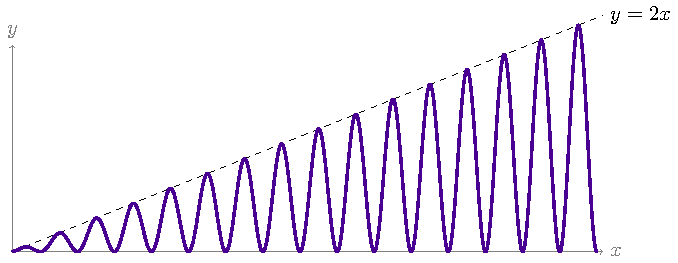
\includegraphics{fig/xsin(x+1).pdf}}
\SetAnswer{Using definition~\eref{text}{def_1_8_1}, prove or disprove the following:
\[\dlimx{\infty} x(\sin x + 1) = \infty\]\color{answercolor}
The statement is false.\vfill

\textbf{Proof:} Let $P=1$, and let $M$ be any positive number. There exists an integer $n$ such that $(2n+1.5)\pi>M$. For $x=(2n+1.5)\pi$, we have both $x>M$ and $x(\sin x + 1)=0\not< P$. 

That is: there exists some $P>0$ such that there is \textit{no} $M>0$ with the property that $x(\sin x +1)>P$ whenever $x>M$. So, $\dlimx{\infty}x(\sin x +1)\neq \infty$.
}



%Q3
\SetQuestion{Using definition~\eref{text}{def_1_8_1}, prove or disprove the following:
\[\dlimx{\infty} x(\sin x+2) = \infty\]}
\SetAnswer{Using definition~\eref{text}{def_1_8_1}, prove or disprove the following:
\[\dlimx{\infty} x(\sin x+2) = \infty\]\color{answercolor}
Note $x(\sin x + 2) \ge x(-1+2)=x$ for all values of $x>0$. So if $x>P$, then $x(\sin x+1) \ge x > P$.\vfill

\textbf{Proof: } For any $P>0$, let $M=P$. Whenever $x>M$, then 
\begin{align*}
x(\sin x +2)& \ge x(-1+2)=x>M=P
\end{align*}
So $\dlimx{\infty}x(\sin x+2) = \infty$.}
\SetAnswer{
\vfill
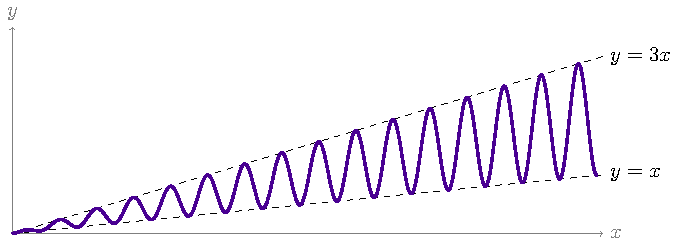
\includegraphics{fig/xsin(x+2).pdf}}

\end{QuestionSet}
\end{frame}

%------------------------------------------------------

%why does M have to be positive?
%% Copyright 2021 Joel Feldman, Andrew Rechnitzer and Elyse Yeager, except where noted.
% This work is licensed under a Creative Commons Attribution-NonCommercial-ShareAlike 4.0 International License.
% https://creativecommons.org/licenses/by-nc-sa/4.0/


%------------------------------------------------------
\section[1.7 Formal Limits]{1.7 (Optional) Making the Informal a Little More Formal}

 \begin{frame}{Table of Contents}
 \begin{center}1.7 (Optional) Making the Informal a Little More Formal
 \end{center}
\mapofcontentsA{}

 \end{frame}
%------------------------------------------------------
%------------------------------------------------------

%------------------------------------------------------

\begin{frame}
Now that we've seen the limits of functions as $x$ goes to positive and negative infinity, let's look at limits as $x$ approaches a real number.
\note{The actual computations for limits as $x$ goes to infinity are generally easier, so I like to teach 1.8 before 1.7.\\[1em]

A lot of the same language from the canning analogy can be re-used here: $\epsilon$ as error, for instance.}
\end{frame}

%------------------------------------------------------

\begin{frame}[t]
\StatusBar{1}{9}
\[\lim_{x \to a} f(x) = L\]
Informally: If $x$ is close enough (but not equal to) $a$, then $y$ is close enough to $L$.

\begin{tikzpicture}

%narrowing intervals
\foreach \x in {1,2,3,4}{
	\MULTIPLY{\x}{2}{\a}
	\ADD{\a}{1}{\b}%slides \a and \b
	%epsilon: 1/2^x
	\POWER{2}{-\x}{\ep}
	\onslide<\a-\b|handout:0>{
		{\color{W1}
		\ifnum \x<4
			\ycoord{1+\ep}{L+\epsilon}
			\ycoord{1-\ep}{L-\epsilon}
		\fi
		\draw[dashed] (.2,1+\ep) -- (4.5,1+\ep) (.2,1-\ep) -- (4.5,1-\ep);
		}}
	%delta: 2*ep^(1/3)
	\EXP[\ep]{0.333}{\da}
	\MULTIPLY{2}{\da}{\d}
	\onslide<\b|handout:0>{
		\fill[W5](2-\d,-0.2) rectangle (1.95,0.2) (2.05,-0.2) rectangle (2+\d,0.2);
		\draw[M5, line width=4pt] plot[domain=2-\d:2+\d,smooth](\x,{(\x/2-1)^3+1});
		\xcoord{2-\d}{a-\delta}
		\xcoord{2+\d}{a+\delta}
		}
	}

\myaxis{x}{1}{4.5}{y}{1}{3}

\draw[C1, thick] plot[domain=-0.52:4.5,smooth](\x,{(\x/2-1)^3+1});
\draw[C1] (2,1)node[thick,opendot]{};
\xcoord{2}{a}
\onslide<-5>{\ycoord{1}{L}}

\end{tikzpicture}
\end{frame}


%------------------------------------------------------

\begin{frame}[t]
\AnswerSpace
\only<2>{\QuestionBar{1}{3}\AnswerYes}
\only<3-5>{\AnswerBar{1}{3}}
\only<6>{\QuestionBar{2}{3}\AnswerYes}
\only<7-8>{\AnswerBar{2}{3}}
\only<9>{\QuestionBar{3}{3}\AnswerYes}
\only<10-11>{\AnswerBar{3}{3}}
Let $f(x) = \begin{cases}
2x & \mbox{ if }x<1\\
4-2x & \mbox{ if }x>1
\end{cases}$. \quad Then 
$\dlimx{1} |x| = 2$.


\begin{multicols}{2}
\begin{tikzpicture}

%narrowing intervals

\onslide<3-5|handout:0>{
	{\color{W1}
	\ycoord{5}{2.5}
	\ycoord{3}{1.5}
	\draw[dashed] (0.2,5)--(4,5) (0.2,3)--(4,3);
}}
\onslide<4-5|handout:0>{
	\xcoord[below left]{1.5}{1-\frac14\!\!\!\!}
	\xcoord[below right]{2.5}{\!\!\!\!1+\frac14}
	\fill[W5] (1.5,-.2) rectangle (1.95,.2) (2.05,-.2) rectangle (2.5,.2);
	\draw[M5,line width=4pt] (1.5,3)--(2,4)--(2.5,3);
	}
%
\onslide<7-8|handout:0>{
	{\color{W1}
	\ycoord{4.5}{2.25}
	\ycoord{3.5}{1.75}
	\draw[dashed] (0.2,4.5)--(4,4.5) (0.2,3.5)--(4,3.5);
}}
\onslide<8|handout:0>{
	\xcoord[below left]{1.75}{1-\frac18\!\!\!}
	\xcoord[below right]{2.25}{\!\!\!1+\frac18}
	\fill[W5] (1.75,-.2) rectangle (1.95,.2) (2.05,-.2) rectangle (2.25,.2);
	\draw[M5,line width=4pt] (1.75,3.5)--(2,4)--(2.25,3.5);
	}

%
\onslide<10-|handout:0>{
	{\color{W1}
	\ycoord{4.3}{2+\epsilon}
	\ycoord{3.7}{2-\epsilon}
	\draw[dashed] (0.2,4.3)--(4,4.3) (0.2,3.7)--(4,3.7);
}}
\onslide<11-|handout:0>{
	\xcoord[below left]{1.85}{1-\frac\epsilon{2}\!\!}
	\xcoord[below right]{2.15}{\!\!1+\frac\epsilon 2}
	\fill[W5] (1.85,-.2) rectangle (1.95,.2) (2.05,-.2) rectangle (2.15,.2);
	\draw[M5,line width=4pt] (1.85,3.7)--(2,4)--(2.15,3.7);
	}


\myaxis{x}{0}{4.1}{y}{0}{5.1}

\draw[C1, thick] (0,0)--(2,4) node[midway,xshift=-3mm,rotate=60]{$y=2x$};
\draw[C1, thick] (2,4)--(4,0) node[midway,xshift=3mm,rotate=-60]{$y=4-2x$};

\draw[C1] (2,4)node[thick,opendot]{};
\xcoord{2}{1}
\ycoord{4}{2}

\end{tikzpicture}
\columnbreak

\color{C1}

\only<2-8>{Find a positive number $\delta$ such that $|f(x)-2|<\alert{\frac12}$ for all $x$ in the interval $(1-\delta,1+\delta)$, except possibly $x=1$.}

\only<5-8|handout:0>{\textcolor{answercolor}{\[\delta = \frac14\]}}


\only<6-8>{Find a positive number $\delta$ such that $|f(x)-2|<\alert{\frac14}$ for all $x$ in the interval $(1-\delta,1+\delta)$, except possibly $x=1$.}

\only<8|handout:0>{\textcolor{answercolor}{\[\delta = \frac18\]}}


\only<9-|handout:0>{Let $\epsilon>0$. Find a positive number $\delta$ such that $|f(x)-2|<\alert{\epsilon}$ for all $x$ in the interval $(1-\delta,1+\delta)$, except possibly $x=1$.}

\only<11-|handout:0>{\textcolor{answercolor}{\[\delta = \frac\epsilon 2\]}}


\end{multicols}
\end{frame}

%------------------------------------------------------

\begin{frame}[t]
\begin{block}{Definition~\eref{text}{def_1_7_1}}
 Let $a \in \mathbb{R}$ and let $f(x)$ be a function defined everywhere in a
neighbourhood of $a$, except possibly at $a$. We say that
\begin{quote}
 the limit as $x$ approaches $a$ of $f(x)$ is $L$
\end{quote}\\
and write
\begin{align*}
  \lim_{x \to a} f(x) &= L
\end{align*}
if and only if for every $\epsilon >0$ there exists $\delta>0$ so that
\begin{align*}
  |f(x) - L| <\epsilon & \text{ whenever } 0<|x-a| < \delta
\end{align*}
Note that an equivalent way of writing this very last statement is
\begin{align*}
  \text{if } 0<|x-a| < \delta \text{ then } |f(x) - L| <\epsilon.
\end{align*}
\end{block}
\end{frame}

%------------------------------------------------------

\begin{frame}[t]
\StatusBar{1}{6}
\begin{tikzpicture}[xscale=2]
\onslide<2->{ \ycoord{1}{L}}
\onslide<3-|handout:0>{
	{\color{W1}
	\ycoord[xshift=-3mm]{.75}{L-\epsilon}
	\ycoord[xshift=-3mm]{1.25}{L+\epsilon}
	\draw[dashed] (0.2,0.75)--(4,0.75) (0.2,1.25)--(4,1.25);
	}}
\onslide<4-|handout:0>{\xcoord[yshift=-2mm]{1.5}{a-\delta} \xcoord[yshift=-2mm]{2.5}{a+\delta} }
\onslide<5-|handout:0>{\fill[W5] (1.55,-.1) rectangle (1.95,0.1) (2.05,-.1) rectangle (2.45,0.1);
	\draw[line width=4pt, M5] plot[domain=1.45:1.95](\x,{0.5+\x/4+0.1*sin(\x*12.566 r)});
	\draw[line width=4pt, M5] plot[domain=2.05:2.45](\x,{0.5+\x/4+0.1*sin(\x*12.566 r)});
	}
%graph
\myaxis{x}{0}{4}{y}{0}{2}
\draw[C1, thick] plot[domain=0.25:3.75,samples=50,smooth](\x,{0.5+\x/4+0.1*sin(\x*12.566 r)})node[right]{$y=f(x)$};
\xcoord{2}{a}
\end{tikzpicture}

\alert<1|handout:0>{ Let $a \in \mathbb{R}$ and let $f(x)$ be a function defined everywhere in a
neighbourhood of $a$, except possibly at $a$. }\pause

\alert<2|handout:0>{We write
\[  \dlimx{a} f(x) = L\]
}\pause
\alert<3|handout:0>{if and only if for every $\epsilon >0$}\pause
\alert<4|handout:0>{ there exists $\delta>0$ }\pause
\alert<5|handout:0>{ so that \[  |f(x) - L| <\epsilon  \text{ whenever } 0<|x-a| < \delta\]
}\pause

\end{frame}

%------------------------------------------------------

\begin{frame}[t]
\only<1>{\AnswerYes\QuestionBar{1}{3}}
\only<2->{\AnswerBar{1}{3}}
\only<1>{\begin{block}{Definition~\eref{text}{def_1_7_1}}
Let $a \in \mathbb{R}$ and let $f(x)$ be a function defined everywhere in a
neighbourhood of $a$, except possibly at $a$. We say that
$  \dlimx{a} f(x) = L$
if and only if for every $\epsilon >0$ there exists $\delta>0$ so that
if $0<|x-a| < \delta$ then $|f(x) - L| <\epsilon$.
\end{block}}

\textcolor{C1}{Using Definition~\eref{text}{def_1_7_1}, prove that $\dlimx{-1}|x+1| = 0$.}\\
\only<2|handout:0>{\color{answercolor}By inspection (look at the graph 
of $y=|x+1|$),  we should use $\delta = \epsilon$.\vfill
Proof: 
Let $f(x)=|x+1|$ and for any positive $\epsilon$, let $\delta = \epsilon$.\\

\begin{center}
\begin{tikzpicture}\color{black}
\draw[line width=4pt,W1] (-2.95,0)--(-0.05,0)node[midway,below]{$-1-\delta \le x \le -1$};
\draw[line width=4pt,M5] (0.05,0)--(2.95,0)node[midway,below]{$-1<x<-1-\delta $};
\draw[<->] (-4,0)--(4,0);
\nxcoord{3}{-1+\delta}
\nxcoord{-3}{-1-\delta}
\nxcoord{0}{-1}
\end{tikzpicture}\end{center}


 If\quad\textcolor{M5}{ $-1<x<-1+\delta$}:
\begin{align*}
|f(x)-0|&=||x+1|-0| = |x+1|=x+1 < (-1+\delta)+1 = \delta =\epsilon
\intertext{If \quad \textcolor{W1}{$-1-\delta<x<-1$}:}
|f(x)-0|&=||x+1|-0| = |x+1|=-x-1 < -(-1-\delta)-1= \delta =\epsilon
\end{align*}

So if $0<|x-(-1)|<\delta$, then $|f(x)-0|<\epsilon$. That is, $  \dlimx{-1} f(x) = 0$.\qed
}
\end{frame}
%%-----------------------------------------
%%------------------------------------------------------
%%------------------------------------------------------

\begin{frame}[t]
\unote{Example~\eref{text}{eg_1_7_1}}
\only<1>{\AnswerYes\QuestionBar{2}{3}}
\only<2->{\AnswerBar{2}{3}}
\only<1>{\begin{block}{Definition~\eref{text}{def_1_7_1}}
 Let $a \in \mathbb{R}$ and let $f(x)$ be a function defined everywhere in a
neighbourhood of $a$, except possibly at $a$. We say that
$  \dlimx{a} f(x) = L$
if and only if for every $\epsilon >0$ there exists $\delta>0$ so that
if $0<|x-a| < \delta$ then $|f(x) - L| <\epsilon$.
\end{block}}
%
\only<1>{
\textcolor{C1}{Let $f(x) = \begin{cases}
x+1 & x <0\\
1-x^2 & x>0
\end{cases}$.\\
Using Definition~\eref{text}{def_1_7_1}, prove that $\dlimx{0}f(x) = 1$.}}
\only<2|handout:0>{
\color{answercolor}
First, we need to find $\delta$ for any given $\epsilon$. Suppose $x>0$ and $|f(x)-1|<\epsilon$:
\begin{align*}
|f(x)-1|&<\epsilon\\
|1-x^2-1|&<\epsilon\\
x^2&<\epsilon\\
0< x&<\sqrt{\epsilon}
\end{align*}
Now, suppose $x<0$ and $|f(x)-1|<\epsilon$:
\begin{align*}
|f(x)-1|&<\epsilon\\
|x+1-1|&<\epsilon\\
|x|&<\epsilon\\
-x&<\epsilon\\
0>x&>-\epsilon
\end{align*}
}
\only<3|handout:0>{
\color{answercolor}
Now we know the interval over which $|f(x)-1|<\epsilon$, but it's actually more information than we need. We don't need the exact interval; we just need some value of $\delta$ such that $0<|x-1|<\delta$ guarantees $|f(x)-1|<\epsilon$.
\begin{center}\begin{tikzpicture}[xscale=2.5]
\draw[M5,line width=4pt] (-.25,.75)-- (0,1) plot[domain=0:.5](\x,{1-\x*\x});
\myaxis{x}{1.5}{1.5}{y}{1.1}{1.25}
\draw[thick,C1] (-1.5,-.5)--(0,1);
\draw[thick,C1] (0,1) node[opendot]{}plot[domain=0:1.5](\x,{1-\x*\x});
\xcoord{.5}{\sqrt{\epsilon}}
\xcoord{-.24}{-\epsilon}
\end{tikzpicture}\end{center}

If $0<|x-1|<\min\{\epsilon,\sqrt \epsilon\}$, then $0<|x-1|<\epsilon$ and 
$0<|x-1|<\sqrt\epsilon$ are both true. So we set $\delta = \min\{\epsilon,\sqrt \epsilon\}$. (For $\epsilon<1$, that is $\delta=\epsilon$.)
}
\only<4|handout:0>{
\color{answercolor}
Proof: $f(x) = \begin{cases}
x+1 & x <0\\
1-x^2 & x>0
\end{cases}$.\\
 For any $\epsilon>0$, let $\delta = \min\{\epsilon,\sqrt{\epsilon}\}$. Suppose $0<|x-0|<\delta$.
\begin{itemize}\color{answercolor}
\item If $x>0$, then
\begin{align*}
|f(x)-1| &= |(1-x^2)-1|=|-x^2|=x^2\\
&<\delta^2\le\sqrt{\epsilon}^2=\epsilon
\end{align*}
\item If $x<0$, then
\begin{align*}
|f(x)-1| &= |(x+1)-1|=|x|\\
&<\delta\le\epsilon
\end{align*}
\end{itemize}
So whenever $0<|x-0|<\delta$, then $|f(x)-1|<\epsilon$. So $\dlimx{0}f(x) = 1$. \qed
}
\end{frame}

%------------------------------------------------------

\begin{frame}[t]{General Principles}
\StatusBar{1}{4}
Suppose $|f(x)-L|<\epsilon$ whenever $a-\delta_1<x<a$ and whenever $a<x<a+\delta_2$.
\begin{center}
\begin{tikzpicture}
\draw[line width=5 pt, M5] plot[domain=3.26:8,smooth](\x,{40/(\x*\x+16)});

\onslide<3-|handout:0>{
	\xcoord[W1]{6.5}{a+\delta_1}
	\draw[line width=3 pt, W1] plot[domain=3.26:6.5,smooth](\x,{40/(\x*\x+16)});
	}


\myaxis{x}{0}{9}{y}{0}{3}
\draw[thick, C1] plot[domain=0:9,smooth](\x,{40/(\x*\x+16)});
\ycoord{1}{L}
\ycoord{1/2}{L+\epsilon}
\ycoord{1.5}{L-\epsilon}
\draw[dashed] (.2,1.5)--(9,1.5) (.2,.5)--(9,.5);
\xcoord{8}{a+\delta_2}
\xcoord{4.88}{a}
\xcoord{3.26}{a-\delta_1}
\draw[C1] (4.88,1)node[opendot]{};

\end{tikzpicture}
\end{center}\pause
Consider values of $x$ such that $0<|x-a|<\min\{\delta_1,\delta_2\}$. 
\onslide<4|handout:0>{For these values, it is (still) the case that $|f(x)-L|<\epsilon$.}

\end{frame}

%------------------------------------------------------

\begin{frame}[t]{General Principles}
\note<1>{WLOG prove only for small epsilon. This doesn't really come up so often at this level, which is why there's a skip button.}
\StatusBar{1}{7}
Suppose $|f(x)-L|<\alert{\frac{1}{10}}$ for all $x$ such that $0<|x-a|<\delta$.\\
\onslide<4-|handout:0>{Then also $|f(x)-L|<\alert{\only<4>{\frac{1}{5}}\only<5>{\frac12}\only<6>{1}\only<7>{100}}$ for all $x$ such that $0<|x-a|<\delta$.}

\begin{center}
\begin{tikzpicture}
\draw[line width=5 pt, M5] plot[domain=3.:6.,smooth](\x,{3-\x/3});
\myaxis{x}{0}{9}{y}{0}{3}
\draw[thick, C1] plot[domain=0.25:8.5,smooth](\x,{3-\x/3});
\ycoord{1.5}{L}
\ycoord{1}{L-\frac{1}{10}}
\ycoord{2}{L+\frac{1}{10}}
\onslide<-2|handout:0>{\draw[dashed] (.2,1)--(9,1) (.2,2)--(9,2);}
\xcoord{6}{a+\delta}
\xcoord{4.5}{a}
\xcoord{3}{a-\delta}
\draw[C1] (4.5,1.5)node[opendot]{};

\onslide<3-4|handout:0>{
	\ycoord{.5}{L-\frac{1}{5}}
	\ycoord{2.5}{L+\frac{1}{5}}
	\draw[dashed] (0.2,.5)--(9,.5) (0.2,2.5)--(9,2.5);
	}
\end{tikzpicture}
\end{center}
\onslide<2-4>{
Can you give values of $x$ where $|f(x)-L|<\alert{\frac{1}{5}}$?}

\vfill\hfill \hyperlink{endWLOG}{\beamerskipbutton{skip $\epsilon$ small}}
\end{frame}
%------------------------------------------------------

\begin{frame}[t]{General Principles}
\begin{block}{Definition~\eref{text}{def_1_7_1}}
 Let $a \in \mathbb{R}$ and let $f(x)$ be a function defined everywhere in a
neighbourhood of $a$, except possibly at $a$. We say that
$  \dlimx{a} f(x) = L$
if and only if \alert{for every $\epsilon >0$} there exists $\delta>0$ so that
if $0<|x-a| < \delta$ then $|f(x) - L| <\epsilon$.
\end{block}\pause

It is enough to show that \alert{for every $\epsilon$ such that $0<\epsilon<c$} (where $c$ is some constant) there exists $\delta>0$ so that
if $0<|x-a| < \delta$ then $|f(x) - L| <\epsilon$.\vfill

That means it doesn't hurt your proof if you say something like ``we assume $\epsilon < 1$".\pause\vfill

In a previous example, we chose
\[\delta = \min\{\epsilon, \sqrt \epsilon\}\]
It would be OK to say ``we can assume $\epsilon<1$; set $\delta = \epsilon$."

\end{frame}

%------------------------------------------------------

\begin{frame}[t]
\label{endWLOG}%end of the section about how we can assume $\epsilon$ is sufficiently small
\only<1>{\AnswerYes\QuestionBar{3}{3}}
\only<2->{\AnswerBar{3}{3}}
\only<1>{\begin{block}{Definition~\eref{text}{def_1_7_1}}
 Let $a \in \mathbb{R}$ and let $f(x)$ be a function defined everywhere in a
neighbourhood of $a$, except possibly at $a$. We say that
$  \dlimx{a} f(x) = L$
if and only if for every $\epsilon >0$ there exists $\delta>0$ so that
if $0<|x-a| < \delta$ then $|f(x) - L| <\epsilon$.
\end{block}}

\only<1>{\textcolor{C1}{Using Definition~\eref{text}{def_1_7_1}, prove that $\dlimx{2}\frac{x-2}{x^2-4} = \frac14$.}}
\only<2|handout:0>{\color{answercolor}\small
\begin{multicols}{2}
We start, as usual, by finding $\delta$. Note
\begingroup
\allowdisplaybreaks
\begin{align*}
\frac{x-2}{x^2-4}=\frac{x-2}{(x+2)(x-2)} &= \frac{1}{x+2}
\intertext{whenever $x\neq 2$.}
\left| \frac{1}{x+2}-\frac14\right|&<\epsilon\\
-\epsilon< \frac{1}{x+2}-\frac14&<\epsilon\\
\frac14-\epsilon< \frac{1}{x+2}&<\frac14+\epsilon\\
\frac{1-4\epsilon}{4}< \frac{1}{x+2}&<\frac{1+4\epsilon}{4}\\
\frac4{1-4\epsilon}> x+2&> \frac4{1+4\epsilon}\\
\frac4{1-4\epsilon}-2> x&> \frac4{1+4\epsilon}-2\\
\frac{2+8\epsilon}{1-4\epsilon}>x&>\frac{2-8\epsilon}{1+4\epsilon}
\intertext{We want our bounds to look like $2-\delta_1$ and $2+\delta_2$.}
\frac{2-8\epsilon+16\epsilon}{1-4\epsilon}>x&>\frac{2+8\epsilon-16\epsilon}{1+4\epsilon}\\
2+\frac{16\epsilon}{1-4\epsilon}>x&>2-\frac{16\epsilon}{1+4\epsilon}
\end{align*}
\endgroup
For $x$ in the interval found, $\left|f(x)-\frac14\right|<\epsilon$. The interval is not exactly in the form $2-\delta < x  <2+\delta$, but it's close. Remember a smaller interval will also have the property $\left|f(x)-\frac14\right|<\epsilon$. So, set \[\delta = \min\left\{\tfrac{16\epsilon}{1-4\epsilon}, \tfrac{16\epsilon}{1+4\epsilon}\right\} =  \tfrac{16\epsilon}{1+4\epsilon}.\]
\end{multicols}
}
\only<3|handout:0>{\color{answercolor}
Proof: For any $\epsilon>0$, let $\delta= \frac{16\epsilon}{1+4\epsilon}$. Suppose $0<|x-2|<\delta$. Note that since $x \neq 2$, we have $f(x) = \frac{x-2}{(x+2)(x-2)}  = \frac{1}{x+2}$.
\begin{itemize}\color{answercolor}
\item If $x>2$, then $2<x<2+\delta$:
\begin{align*}
\left|f(x) - \frac14\right|& =
\left|\frac{1}{(x+2)} - \frac14\right| = \frac14-\frac{1}{(x+2)}\\
&<\frac14-\frac{1}{(2+\delta)+2} = \frac14-\frac{1}{4+\delta} \\
&=\frac14-\frac{1}{4+\frac{16\epsilon}{1+4\epsilon}}<\frac14-\frac{1}{4+\frac{16\epsilon}{1-4\epsilon}}
\intertext{(using the fact that $\delta= \frac{16\epsilon}{1+4\epsilon}<\frac{16\epsilon}{1-4\epsilon}$)}
&=\frac14-\frac{1}{\frac{4-16\epsilon+16\epsilon}{1-4\epsilon}} = \frac14 - \frac{1-4\epsilon}{4} = \frac{4\epsilon}{4}=\epsilon
\end{align*}
\end{itemize} 
}
\only<4|handout:0>{\color{answercolor}
\begin{itemize}\color{answercolor}
\item If $x<2$, then $2-\delta<x<2$:
\begin{align*}
\left|f(x) - \frac14\right|& =
\left|\frac{1}{(x+2)} - \frac14\right| =\frac{1}{(x+2)}- \frac14\\
&<\frac{1}{(2-\delta)+2}- \frac14 =\frac{1}{4-\delta} - \frac14\\
&=\frac{1}{4-\frac{16\epsilon}{1+4\epsilon}}-\frac14
=\frac{1}{\frac{4+16\epsilon-16\epsilon}{1+4\epsilon}}-\frac14\\
& = \frac{1+4\epsilon}4-\frac14 = \epsilon
\end{align*}
We have shown that whenever $0<|x-2|<\delta$, then $\left|f(x)-\frac14\right|<\epsilon$. So,
$\dlimx{2}\frac{x-2}{x^2-4} = \frac14$.
\end{itemize} \qed
}

\end{frame}
%------------------------------------------------------

%------------------------------------------------------

\begin{frame}[t]{Infinite Limits}
\begin{block}{Definition~\eref{text}{def_1_8_1} (b)}
Let $a$ be a real number and $f(x)$ be a function defined for all $x \neq a$. We write
\[\lim_{x \to a}f(x) = \infty\]
if and only if for every \alert<2|handout:0>{$P>0$} there exists \alert<3|handout:0>{$\delta>0$} so that \alert<4|handout:0>{$f(x)>P$ whenever $0<|x-a|<\delta$}.
\end{block}


\begin{tikzpicture}
\myaxis{x}{0}{4}{}{0}{2.5}
\xcoord{2}{a}

\onslide<2-|handout:0>{\ycoord{2}{\alert<2>{P}}\draw[dashed] (.2,2)--(4,2);}
\onslide<3-|handout:0>{\xcoord[xshift=4mm]{2.25}{\alert<3>{a+\delta}}\xcoord[xshift=-4mm]{1.75}{\alert<3>{a-\delta}}}
\onslide<4-|handout:0>{\draw[M5,line width=4pt] plot[domain=2.16:2.25,smooth](\x,{1/(sqrt(\x-2))});
\draw[M5,line width=4pt] plot[domain=1.75:1.84,smooth](\x,{1/(sqrt(2-\x))});
}

\draw[C1,thick] plot[domain=2.16:4,smooth](\x,{1/(sqrt(\x-2))});
\draw[C1,thick] plot[domain=0:1.84,smooth](\x,{1/(sqrt(2-\x))});
\end{tikzpicture}
\end{frame}



%------------------------------------------------------

\begin{frame}[t]
\AnswerSpace
\begin{block}{Definition~\eref{text}{def_1_8_1} (b)}
Let $a$ be a real number and $f(x)$ be a function defined for all $x \neq a$. We write
\[\lim_{x \to a}f(x) = \infty\]
if and only if for every $P>0$ there exists $\delta>0$ so that $f(x)>P$ whenever $0<|x-a|<\delta$.
\end{block}


\begin{multicols}{2}
\note<1>{The generic picture is kept on the left, but it's nice to mention that it is, indeed, generic. In particular, the picture won't fit for $f(x) = \frac{1}{x-2}$.}
\begin{QuestionSet}
%Q1
\SetQuestion{\begin{tikzpicture}
\myaxis{x}{0}{4}{}{0}{2.5}
\ycoord{2}{P}\draw[dashed] (.2,2)--(4,2);
\xcoord[xshift=4mm]{2.25}{3+\delta}\xcoord[xshift=-4mm]{1.75}{3-\delta}
\draw[M5,line width=4pt] plot[domain=2.16:2.25,smooth](\x,{1/(sqrt(\x-2))});
\draw[M5,line width=4pt] plot[domain=1.75:1.84,smooth](\x,{1/(sqrt(2-\x))});


\draw[C1,thick] plot[domain=2.16:4,smooth](\x,{1/(sqrt(\x-2))});
\draw[C1,thick] plot[domain=0:1.84,smooth](\x,{1/(sqrt(2-\x))});
\end{tikzpicture}
\columnbreak

Let $f(x) = \frac{1}{(x-3)^2}$. Using Definition~\eref{text}{def_1_8_1}, prove or disprove that
\[\dlimx{3}f(x)=\infty\]
\AnswerYes\MoreSpace}
\SetAnswer{\AnswerYes}
\SetAnswer{\color{answercolor}
First, we find $\delta$.  Let $P>0$.
\begin{align*}
f(x)&>P\\
\frac{1}{(x-3)^2}&>P\\
(x-3)^2&<\frac1P\\
|x-3|&<\frac1{\sqrt P}
\end{align*}
So we choose $\delta = \frac1{\sqrt P}$. 
}
\SetAnswer{
\color{answercolor}
\textbf{Proof: } For any $P>0$, set $\delta = \frac1{\sqrt P}$. If $0<|x-3|$, then $x \neq 3$, so $f(x)$ exists. If, furthermore, $|x-3|<\delta$, then: 
\abovedisplayshortskip=0pt
\begin{align*}
f(x)&=\frac{1}{(x-3)^2} \\
&>\frac{1}{\delta^2}
=\frac{1}{\left(\frac{1}{\sqrt P}\right)^2}
=P
\end{align*}
\columnbreak

So, $\dlimx{3}\frac{1}{(x-3)^2} = \infty$.

}

%Q2
\SetQuestion{Let $f(x) = \frac{1}{x-2}$. Using Definition~\eref{text}{def_1_8_1}, prove or disprove that
\[\dlimx{2}f(x)=\infty\]
\columnbreak
\AnswerYes\MoreSpace}
\SetAnswer{\AnswerYes}
\SetAnswer{\color{answercolor}
Note that $x-2<0$ when $x<2$. So for any $P>0$, whenever $x<2$, we have $f(x)<P$. That tells us that $\dlimx{2}f(x)\neq\infty$.\columnbreak

\textbf{Proof: } Let $P=1$. For any $\delta>0$, set $x_0=2-\frac{\delta}{2}$. Then $0<|x_0-2|<\delta$, but since $x<2$, we have $\frac{1}{x-2}<0<P$. That is, there does not exist any $\delta>0$ such that $f(x)>P$ whenever $0<|x-2|<\delta$. Therefore $\dlimx{2}f(x)\neq\infty$.}
\SetAnswer{
\begin{tikzpicture}
\myaxis{x}{0}{4}{}{2}{2}
\draw[thick,C1]plot[domain=0:1.5](\x,{1/(\x-2)});
\draw[thick,C1]plot[domain=2.5:4](\x,{1/(\x-2)});
\xcoord{2}{2}
\end{tikzpicture}
}

\end{QuestionSet}
\end{multicols}
\end{frame}


%------------------------------------------------------


%%chapter 2
\foreach \n in {1,2,3,4,7,8,9,10,11,12,13,14}{
\input{sections/2_\n.tex}
}
%%chapter 3
\foreach \n in {1,...,7}{
\input{sections/3_\n.tex}
}
%chapter 4
% Copyright 2021 Joel Feldman, Andrew Rechnitzer and Elyse Yeager, except where noted.
% This work is licensed under a Creative Commons Attribution-NonCommercial-ShareAlike 4.0 International License.
% https://creativecommons.org/licenses/by-nc-sa/4.0/


%----------------------------------------------------------------------------------------
%----------------------------------------------------------------------------------------
\section*{4.1: Antiderivatives}
%----------------------------------------------------------------------------------------
%----------------------------------------------------------------------------------------
%----------------------------------------------------------------------------------------

%----------------------------------------------------------------------------------------
%----------------------------------------------------------------------------------------
\begin{frame}
\centering\Large
4.1 Antiderivatives
\end{frame}
%----------------------------------------------------------------------------------------
\begin{frame}[t]
\unote{Definition~\eref{text}{def:antiderivative}}
\AnswerSpace
\only<4>{\AnswerYes}
\begin{block}
{Basic Question}
What function has derivative $f(x)$?
\end{block}
\pause\vfill

If $F'(x)=f(x)$, we call $F(x)$ an \textcolor{M4}{antiderivative} of $f(x)$.\pause\vfill

\begin{block}
{Examples}
$\diff{}{x}[x^2]=2x$, so $x^2$ is an \emph{antiderivative} of $2x$.
\vspace{5mm}

$\diff{}{x}[x^2+5]=2x$, so $x^2+5$ is (also) an \emph{antiderivative} of $2x$.
\end{block}
\pause\vfill

What is the most general antiderivative of $2x$? \\\color{answercolor}
\pause \answer{\fbox{$x^2+c$}, where we understand $c$ as some constant \\(a number not depending on $x$).}
\end{frame}
%----------------------------------------------------------------------------------------

%----------------------------------------------------------------------------------------
\begin{frame}[t]{Antiderivatives}
Find the most general antiderivative for the following equations.
\[f(x)= 17\]
\onslide<2|handout:0>{\textcolor{answercolor}{$17x+c$}}
\vfill
\[f(x)= m \] where $m$ is a constant.

\onslide<2|handout:0>{\textcolor{answercolor}{$mx+c$}}
\vfill
\note<1>{This is a good time to remind students about lines.}
\end{frame}
%----------------------------------------------------------------------------------------
%----------------------------------------------------------------------------------------
\begin{frame}
\StatusBar{1}{7}
\only<1-6>{\AnswerYes}

	\begin{tabular}{lcl}
		differentiation fact && antidifferentiation fact\\ \hline
		$\diff{}{x}[x^2]=2x$ &$\implies$&antideriv of $2x:$\hfill \answer{$ x^2+c$} \\[10pt] \pause
\iftoggle{printsolutions}{		&&antideriv of $x$:\hfill\pause\answer{$\frac{1}{2}x^2+c$}\\[10pt] \pause
		&&\textcolor{W1}{Check: $\diff{}{x}\left[\frac{1}{2}x^2+c \right]=\pause x$}\pause\\[1em]}{}
		$\diff{}{x}[x^3]=3x^2$ &$\implies$&
		\onslide<7-|handout:0>{antideriv of $3x^2$:\hfill $x^3+c$ \\
		&&antideriv of $ x^2$:}\hfill
		\onslide<7-|handout:0>{ $\frac{1}{3}x^3+c$ }
		\\[10pt]
		$\diff{}{x}[x^4]=4x^3$ &$\implies$& \onslide<7-|handout:0>{antideriv of $4x^3$:\hfill $x^4+c$		
 \\
		&&antideriv of $x^3$\hfill\onslide<7-|handout:0>{$\frac14x^4+c}$\\[1em]}
		$\diff{}{x}[x^5]=5x^4$ &$\implies$& \onslide<7-|handout:0>{antideriv of $5x^4$: \hfill$x^5+c$		
 \\
		&&antideriv of $ x^4$:\hfill
		\onslide<7-|handout:0>{ $\frac{1}{5}x^5+c$ }\\[1em]}
	&& antideriv of $ x^n$:\hfill \onslide<7-|handout:0>{ $\frac{1}{n+1}x^{n+1}+c$\\[1em]}
	\onslide<7-|handout:0>{	&& \color{W1}Check: $\diff{}{x}\left[\frac{1}{n+1}x^{n+1}+c \right]=$\pause $x^n$}
		\end{tabular}
\end{frame}
%----------------------------------------------------------------------------------------
\begin{frame}\AnswerNo
\foreach \x in {1,2,3}{\QuestionBar{\x}{5}}
\begin{block}{Power Rule for Antidifferentiation}
	The most general antiderivative of $x^n$ is $\dfrac{1}{n+1}x^{n+1}+c $
	if $n \neq -1$
	\end{block}\vfill

\begin{itemize}
\item $\ds\diff{}{x}\Big[ \hspace{2cm}\Big]=x^5$\\[2em]
\item $\ds\diff{}{x}\Big[ \hspace{2cm}\Big]=x^3$\\[2em]
\item $\ds\diff{}{x}\Big[ \hspace{2cm}\Big]=\frac12x^3$
\end{itemize}
\end{frame}
%----------------------------------------------------------------------------------------
\begin{frame}\AnswerNo
\unote{Example~\eref{text}{eg antidiff poly}}
\foreach \x in {4,5}{\QuestionBar{\x}{5}}

\begin{block}{Power Rule for Antidifferentiation}
	The most general antiderivative of $x^n$ is $\dfrac{1}{n+1}x^{n+1}+c $
	if $n \neq -1$
	\end{block}\vfill

\begin{itemize}
\item $\ds\diff{}{x}\Big[ \hspace{4cm}\Big]=5x^2-15x+3 $\\[2em]
\item $\ds\diff{}{x}\Big[ \hspace{4cm}\Big]=13\left(5x^{14}-3x^{3/7}+52e^x\right)$
\end{itemize}
\note{Now is a good time to remind students that power functions and exponential functions aren't the same}
\end{frame}
%----------------------------------------------------------------------------------------
%----------------------------------------------------------------------------------------
\begin{frame}[t]
\only<1>{\QuestionBar{1}{3}\AnswerYes}
\only<2>{\AnswerBar{1}{3}}
Find the most general antiderivatives.
\[f(x)= \cos x\]
\onslide<2|handout:0>{\textcolor{answercolor}{$\sin x+c$}}
\vfill 

\[f(x)= \sin x \]\onslide<2|handout:0>{\textcolor{answercolor}{$-\cos x+c$}}
\vfill

\[f(x)= \sec^2 x\]\onslide<2|handout:0>{\textcolor{answercolor}{$\tan x+c$}}
\vfill

\[f(x)= \frac{1}{1+x^2} \]\onslide<2|handout:0>{\textcolor{answercolor}{$\arctan x +c$}}
\vfill

\[f(x)=\frac{1}{1+x^2+2x}\]
\onslide<2|handout:0>{\textcolor{answercolor}{$\frac{-1}{x+1}$}}
\vfill
\end{frame}
%----------------------------------------------------------------------------------------
%----------------------------------------------------------------------------------------
\begin{frame}[t]
\only<1>{\QuestionBar{2}{3}\AnswerYes}
\only<2>{\AnswerBar{2}{3}}

Find the most general antiderivatives.
\[f(x)= 17\cos x+x^5\]\onslide<2|handout:0>{\textcolor{answercolor}{$17\sin x +\frac{1}{6}x^6+c$}}
\vfill 

\[f(x) =\frac{23}{5+5x^2} \]\onslide<2|handout:0>{\textcolor{answercolor}{$\frac{23}{5}\arctan x +c$}}
\vfill

\[f(x)=\frac{23}{5+125x^2}\]\onslide<2|handout:0>{\textcolor{answercolor}{$\frac{23}{25}\arctan (5x) +c$}}
\vfill
\note<1>{Not all of these are to actually do -- more to show that there can be trickiness, and that trickiness will be a big part of next semester. Let students work on them in order, only the fastest students will get to the last examples on each slide.}
\end{frame}
%----------------------------------------------------------------------------------------
%----------------------------------------------------------------------------------------
\begin{frame}[t]
\only<1>{\QuestionBar{3}{3}\AnswerYes}
\only<2>{\AnswerBar{3}{3}}

Find the most general antiderivatives.
\[f(x)=\frac{1}{x}, ~x>0\]\onslide<2|handout:0>{\textcolor{answercolor}{$\ln x+c$}}
\vfill 

\[f(x)= 5x^2-32x^5-17\]\onslide<2|handout:0>{\textcolor{answercolor}{$\frac{5}{3}x^3-\frac{16}{3}x^6-17x+c$}}
\vfill

\[f(x)=\csc x \cot x \]\onslide<2|handout:0>{\textcolor{answercolor}{$-\csc x+c$}}
\vfill

\[f(x)=\frac{5}{\sqrt{1-x^2}}+ 17\]\onslide<2|handout:0>{\textcolor{answercolor}{$5\arcsin x + 17x +c$}}
\vfill
\end{frame}
%----------------------------------------------------------------------------------------
%----------------------------------------------------------------------------------------
\begin{frame}[t]{Chose Your Own Adventure}
\only<1>{\QuestionBar{1}{7}\AnswerYes}
\only<2>{\AnswerBar{1}{7}}
\only<3>{\QuestionBar{2}{7}\AnswerYes}
\only<4>{\AnswerBar{2}{7}}
Antiderivative of \textcolor{M3}{$ \sin x \cos x $}:
\begin{itemize}
\item[A.] $\cos x\sin x+c$
\item[B.] $-\cos x\sin x+c$
\item[C.] $\sin^2 x+c$
\alert<2-|handout:0>{\item[D.] $\frac{1}{2}\sin^2 x +c$}
\item[E.] $\frac{1}{2}\cos^2x\sin^2x+c$
\end{itemize}\vfill

\onslide<3->{
In general, antiderivatives of $x^n$ have the form $\frac{1}{n+1}x^{n+1}$. What is the single exception?
\begin{itemize}
\alert<4|handout:0>{\item[A.] $n=-1$}
\item[B.] $n=0$
\item[C.] $n=1$
\item[D.] $n=e$
\item[E.] $n=1/2$
\end{itemize}
}\vfill
\end{frame}
%----------------------------------------------------------------------------------------
%----------------------------------------------------------------------------------------
%----------------------------------------------------------------------------------------
\begin{frame}[t]{All the Adventures are Calculus, Though}
\only<1>{\QuestionBar{3}{7}\AnswerYes}
\only<2>{\AnswerBar{3}{7}}
\only<3>{\QuestionBar{4}{7}\AnswerYes}
\only<4>{\AnswerBar{4}{7}}

Suppose the velocity of a particle at time $t$ is given by $v(t)=t^2+\cos t + 3$. What function gives its position?
\begin{itemize}
\item[A.] $s(t)=2t-\sin t $
\item[B.] $s(t)=2t-\sin t +c$
{\item[C.] $s(t)=t^3+\sin t +3t +c$}
\alert<2-|handout:0>{\item[D.] $s(t)=\frac{1}{3}t^3+\sin t +3t +c$}
\item[E.] $s(t)=\frac{1}{3}t^2-\sin t +3t +c$
\end{itemize}
\vfill
\onslide<3->{
Suppose the velocity of a particle at time $t$ is given by $v(t)=t^2+\cos t + 3$, and its position at time 0 is given by $s(0)=5$. What function gives its position?
\begin{itemize}
\item[A.]  $s(t)=\frac{1}{3}t^3+\sin t +3t $
\alert<4-|handout:0>{\item[B.]  $s(t)=\frac{1}{3}t^3+\sin t +3t +5$}
{\item[C.] $s(t)=\frac{1}{3}t^3+\sin t +3t +c$}
{\item[D.] $s(t)=5t+c$}
\item[E.] $s(t)=5t+5$
\end{itemize}
}
\end{frame}
%----------------------------------------------------------------------------------------
%----------------------------------------------------------------------------------------
\begin{frame}[t]
\only<1>{\QuestionBar{5}{7}\AnswerYes}
\only<2>{\AnswerBar{5}{7}}

Find all functions $f(x)$ with $f(1)=5$ and $f'(x)=e^{3x+5}$.\pause\vfill
\color{answercolor}

\answer{Antiderivative of $ e^{3x+5}$ is $\frac{1}{3}e^{3x+5}+c$. So we only need to solve for $c$. 

\[5=f(1) = \frac{1}{3}e^{3+5}+c\] implies

\[c=5-\frac{e^8}{3}\]

So 
\[f(x)=\frac{1}{3}e^{3x+5}+5-\frac{e^8}{3}\]}
\end{frame}
%----------------------------------------------------------------------------------------
%----------------------------------------------------------------------------------------
\begin{frame}[t]
\unote{Example~\eref{text}{eg_4_1_2}}
\only<1>{\QuestionBar{6}{7}\AnswerYes}
\only<2>{\AnswerBar{6}{7}}

Let $Q(t)$ be the amount of a radioactive isotope in a sample. Suppose the sample is losing $50 e^{-5t}$ mg per second to decay. If $Q(1)=10{e^{-5}}$mg, find the equation for the amount of the isotope at time $t$.\pause\color{answercolor}\vfill

\answer{
We have 
\[\frac{dQ}{dt} = -50e^{-5t}\] 
Note the negative, since our sample is getting smaller. 

\medskip
Then antidifferentiating, we find $Q(t)=10e^{-5t}+c$ for some constant $c$.

\medskip
 Then since $Q(1)=10e^{-5}$, we see $c=0$.
\vfill
\[\boxed{Q(t)=10e^{-5t}}\]\vfill}
\end{frame}
%----------------------------------------------------------------------------------------
%----------------------------------------------------------------------------------------
\begin{frame}[t]
\only<1>{\QuestionBar{7}{7}\AnswerYes}
\only<2>{\AnswerBar{7}{7}}

Suppose $f'(t)=2t+7$. What is $f(10)-f(3)$?\pause\color{answercolor}\vfill

\answer{From antidifferentiation, we have $f(t)=t^2+7t+c$. Then 
\[f(10)-f(3) = [100+70+c] -[9+21 +c]=170-30=140\]}
\vfill
\end{frame}
%----------------------------------------------------------------------------------------


%----------------------------------------------------------------------------------------
%----------------------------------------------------------------------------------------

%----------------------------------------------------------------------------------------
% Copyright 2021 Joel Feldman, Andrew Rechnitzer and Elyse Yeager, except where noted.
% This work is licensed under a Creative Commons Attribution-NonCommercial-ShareAlike 4.0 International License.
% https://creativecommons.org/licenses/by-nc-sa/4.0/


%----------------------------------------------------------------------------------------
%----------------------------------------------------------------------------------------

%----------------------------------------------------------------------------------------
\begin{frame}
\note{In 2015, there were 6 quizzes during the semester. Their questions are compiled here as a short semester review.

You can show the questions one-by-one by scrolling to the Solutions section.}

This file contains questions spanning CLP-1. It should not be taken as a complete review of the course, but rather as a jumping-off point. If you struggle with one question, go back to review its entire section. Sections are noted at the bottom of each page.
\end{frame}
%----------------------------------------------------------------------------------------


%link to solution
%#1: S or L
%#2: number
\newcommand{\slink}[2]{\hyperlink{sol#1#2}{\beamergotobutton{solution~#1#2}}}
%----------------------------------------------------------------------------------------
%----------------------------------------------------------------------------------------
%----------------------------------------------------------------------------------------
\mode<beamer>{
\section{Questions}
%----------------------------------------------------------------------------------------
%----------------------------------------------------------------------------------------
%----------------------------------------------------------------------------------------

\begin{frame}[t]{Short Answer}
\AnswerYes
\begin{enumerate}[S1.]
\item \label{S1} Find all solutions to $\ds x^3 - 3x^2 - x + 3 =0$
\hfill \slink{S}{1}
\vfill
%
\item  \label{S2} Compute the limit\quad $\ds \lim_{x \to 2} \frac{x-2}{x^2-4}$ \hfill \slink{S}{2}
\vfill
%
\item  \label{S3}  Find all values of $c$ such that the following function is \hfill\slink{S}{3}\\
 continuous:
\[f(x)=\left\{\begin{array}{ccc}
8-cx & \text{if} & x\le c\\
x^2 &  \text{if} & x> c
\end{array}\right.\]
Use the definition of continuity to justify your answer.
\vfill
%
\item  \label{S4} Compute \hfill \slink{S}{4}
$$\lim_{x\to -\infty} \frac{3x+5}{\sqrt{x^2+5}-x}$$
%
\end{enumerate}
\end{frame}
%----------------------------------------------------------------------------------------
\begin{frame}[t]{Short Answer}
\begin{enumerate}[S1.]
\setcounter{enumi}{4}

\item   \label{S5}  Find the equation of the tangent line to the graph of \hfill\slink{S}{5}\
$y=\cos(x)$ at
$x=\dfrac{\pi}{4}$.
\vfill
%
\item  \label{S6}  For what values of $x$ does the derivative of\hfill \slink{S}{6}\\
$\dfrac{\sin(x)}{x^2+6x+5}$ exist?\vfill
\item  \label{S7} Find $f'(x)$ if $f(x)= (x^2+1)^{\sin(x)}$. \hfill\slink{S}{7}
\vfill
%
\item  \label{S8} Consider a function of the form $f(x) = A e^{kx}$ where \hfill\slink{S}{8}\\
$A$ and $k$ are constants. 
If $f(0)=3$ and $f(2)=5$, \\find the constants $A$ and $k$.

\vfill
\end{enumerate}
\end{frame}
%----------------------------------------------------------------------------------------
\begin{frame}[t]{Short Answer}
\begin{enumerate}[S1.]
\setcounter{enumi}{8}

%
\item \label{S9}  Consider a function $f(x)$ which has $f'''(x)=\dfrac{x^3}{10-x^2}$.
Show 
that when we approximate $f(1)$ using its second Maclaurin polynomial, the 
absolute error is less than $\frac{1}{50}=0.02$.   \hfill\slink{S}{9}
\vfill
%
\item  \label{S10}  Estimate $\sqrt{35}$ using a linear approximation   \hfill\slink{S}{10}
\vfill
%
\item \label{S11}  Let $f(x)=x^2-2\pi x - \sin(x)$. Show that there exists a real number $c$ such that $f'(c)=0$.
  \hfill\slink{S}{11}
\vfill
%
\item  \label{S12}  Find the intervals where $f(x)=\frac{\sqrt{x}}{x+6}$ is increasing.
  \hfill\slink{S}{12}
\vfill
%
\end{enumerate}
\end{frame}
%----------------------------------------------------------------------------------------

\begin{frame}{Long Answer}
\AnswerYes
\begin{enumerate}[L1.]
\item  \label{L1}
Compute the limit $\ds \lim_{x\to 1} \frac{\sqrt{x+2}-\sqrt{4-x}}{x-1}$. \hfill\slink{L}{1}
\vfill

\item \label{L2}
Show that there exists at least one real number $c$ such that
$2\tan(c)=c+1$.  \hfill\slink{L}{2}
\vfill

\item \label{L3}
Determine whether the derivative of following function exists at
$x=0$
\begin{align*}
f(x) &=\begin{cases}
  2x^3-x^2 & \text{ if }  x\le 0\\
  x^2\sin\left(\dfrac{1}{x}\right) & \text{ if } x> 0
\end{cases}
\end{align*}
You must justify your answer using the definition of a derivative.

 \hfill\slink{L}{3}
\vfill
\end{enumerate}
\end{frame}
%----------------------------------------------------------------------------------------
\begin{frame}{Long Answer}
\AnswerYes
\begin{enumerate}[L1.]
\setcounter{enumi}{3}
\item \label{L4}
If $x^2\cos(y)+2xe^y = 8$, then find $y'$ at the points where $y=0$.
You must justify your answer.
 \hfill\slink{L}{4}
\vfill

\item \label{L5}
Two particles move in the cartesian plane. Particle A travels on the $x$-axis 
starting at  $(10,0)$ and moving towards the origin with a speed of $2$ units 
per second. Particle B travels on the $y$-axis starting at $(0,12)$ and moving 
towards the origin with a speed of $3$ units per second. What is the rate of 
change of the distance between the two particles when particle A reaches the 
point $(4,0)$?  \hfill\slink{L}{5}
\vfill

\item \label{L6}
Find the global maximum and the global minimum for $f(x)=x^3 - 6x^2 + 2$ on the interval $[3,5]$.
 \hfill\slink{L}{6}
\vfill
\end{enumerate}
\end{frame}
%----------------------------------------------------------------------------------------
%----------------------------------------------------------------------------------------
\section{Solutions}
%----------------------------------------------------------------------------------------
\begin{frame}
\huge\centering
Solutions
\end{frame}
}%%%end of section that only shows up in beamer mode
\mode<handout>{\section{Short Answer}}
%----------------------------------------------------------------------------------------
%----------------------------------------------------------------------------------------
\newcounter{questionnumber}
\setcounter{questionnumber}{1}
%----------------------------------------------------------------------------------------
\newcommand{\qbox}[3]{
	\label{sol#1#2}
	\rule{\textwidth}{1pt}\\
	%
	\mode<beamer>{\hfill \hyperlink{#1#2}{\beamerreturnbutton{back to questions}}\\
	#1\ref{#1#2}.}
	%
	\mode<handout>{
	#1\thequestionnumber
	\stepcounter{questionnumber}}
	%
	\quad #3 \\[1em]
	\rule{\textwidth}{1pt}
	}
%1st argument: long or short
%2nd argument: number
%3rd argument: text
%----------------------------------------------------------------------------------------
%----------------------------------------------------------------------------------------

\begin{frame}[t]
\qbox{S}{1}{Find all solutions to $\ds x^3 - 3x^2 - x + 3 =0$}

\onslide<2-|handout:0>{\textcolor{answercolor}{
\begin{align*}
x^3-3x^2-x+3&=x^2(x-3)-(x-3)\\
&=(x^2-1)(x-3)\\
&=(x+1)(x-1)(x-3)
\end{align*}
The solutions are $x=1$, $x=3$, and $x=-1$.}
\vfill
\unote{Factoring functions is a high-school review topic. It comes in especially handy in Section~\eref{text}{sec curve sketch}, Sketching Graphs}}
\end{frame}
%----------------------------------------------------------------------------------------
\begin{frame}[t]
\qbox{S}{2}{ Compute the limit\quad $\ds \lim_{x \to 2} \frac{x-2}{x^2-4}$}

 \vfill
 \onslide<2-|handout:0>{\textcolor{answercolor}{
 \[\dlimx{2}\frac{x-2}{x^2-4}=\dlimx{2}\frac{x-2}{(x-2)(x+2)}=\dlimx{2}\frac{1}{x+2}=\frac{1}{4}\]}
 \vfill
 }
\unote{ Section~\eref{text}{sec_1_4}: Calculating Limits with Limit Laws}
\end{frame}
%----------------------------------------------------------------------------------------
\begin{frame}[t]\footnotesize
\qbox{S}{3}{
 Find all values of $c$ such that the following function is continuous:
\[f(x)=\left\{\begin{array}{ccc}
8-cx & \text{if} & x\le c\\
x^2 &  \text{if} & x> c
\end{array}\right.\]
Use the definition of continuity to justify your answer.
}
\vfill
\onslide<2-|handout:0>{\color{answercolor}\normalsize
When $x \neq c$, $f(x)$ is continuous. The only difficult spot is when $x=c$. 
\begin{itemize}\color{answercolor}
\item $f(c)=8-c^2$
\item $\dlimx{c^-}f(x)=\dlimx{c^-}(8-cx)=8-c^2$
\item $\dlimx{c^+}f(x)=\dlimx{c^+}(x^2)=c^2$
\end{itemize}
Since $f(x)$ is continuous at $c$ only if $f(c)=\dlimx{c}f(x)$, we see the only values of $c$ that make $f$ continuous are those that satisfy $c^2=8-c^2$. That is, $c=\pm2$.
}
\unote{ Section~\eref{text}{sec_1_6}: Continuity}
\end{frame}

%----------------------------------------------------------------------------------------

\begin{frame}[t]\footnotesize
\qbox{S}{4}{
Compute
$$\lim_{x\to -\infty} \frac{3x+5}{\sqrt{x^2+5}-x}$$}
\vfill
\onslide<2-|handout:0>{\color{answercolor}
We start by factoring out $x$ from both the top and the bottom. 
\begin{align*}
\lim_{x \to - \infty} \frac{3x+5}{\sqrt{x^2+5}-x}\left(\frac{1/x}{1/x}\right)&=\lim_{x \to -\infty}\frac{3+\frac5x}{\frac1x\sqrt{x^2+5}-1}
\intertext{Since $x$ is approaching negative infinity, we can assume $x<0$. Then $x=-|x|=-\sqrt{x^2}$. We'll use this form to push the $\frac1x$ into the square root.}
&=\lim_{x \to -\infty}\frac{3+\frac5x}{-\frac1{\sqrt{x^2}}\sqrt{x^2+5}-1}\\
&=\lim_{x \to -\infty}\frac{3+\frac5x}{-\sqrt{1+\frac{5}{x^2}}-1}
=\frac{3+0}{-\sqrt1-1}= -\frac32
\end{align*}
}
\unote{
Section~\eref{text}{sec_1_5}: Limits at Infinity}
\end{frame}

%----------------------------------------------------------------------------------------

\begin{frame}[t]\small
\qbox{S}{5}{
 Find the equation of the tangent line to the graph of $y=\cos(x)$ at
$x=\dfrac{\pi}{4}$.}

\onslide<2-|handout:0>{
\color{answercolor}
\setlength{\abovedisplayskip}{0 pt}
\begin{align*}
f(x)&= \cos x & f\left(\frac\pi4\right)&=\frac{1}{\sqrt 2}\\
f'(x)&=-\sin x & f'\left(\frac\pi4\right)&=-\frac{1}{\sqrt 2}
\end{align*}
Recall the equation of the tangent line to $y=f(x)$ at $x=a$ is $y=f(a)+f'(a)(x-a)$

\[y=\frac1{\sqrt 2}-\frac{1}{\sqrt 2}\left(x-\frac\pi4\right)\]
}
\unote{
 Section~\eref{text}{sec_2_1}: Revisiting Tangent Lines \qquad
Section~\eref{text}{sec diff trig}: Derivatives of Trigonometric Functions}

\end{frame}
%----------------------------------------------------------------------------------------

\begin{frame}[t]
\qbox{S}{6}{
 For what values of $x$ does the derivative of
$\dfrac{\sin(x)}{x^2+6x+5}$ exist? 
}\vfill

\onslide<2-|handout:0>{
\color{answercolor}
First, note that $x^2+6x+5 = (x+1)(x+5)$, % and that both $\sin(-1)$ and $\sin(-5)$ are nonzero. 
so the function does not exist at either $x=-1$ or $x=-5$. For other values of $x$, using the quotient rule, we see
\[
f'(x)=\frac{(x^2+6x+5)(\cos x) - \sin x (2x+6)}{(x^2+6x+5)^2}\]
which exists over the domain of $f(x)$.
\vfill
All together, the derivative exists for all values of $x$ except $-1$ and $-5$.
\vfill}

\unote{Section~\eref{text}{sec_2_6}: Using the Arithmetic of Derivatives}
\end{frame}
%----------------------------------------------------------------------------------------

%----------------------------------------------------------------------------------------
%----------------------------------------------------------------------------------------
%----------------------------------------------------------------------------------------
\begin{frame}[t]\small
\qbox{S}{7}{Find $f'(x)$ if $f(x)= (x^2+1)^{\sin(x)}$.}
\vfill

\onslide<2-|handout:0>{
\color{answercolor}
$f(x)$ is neither an exponential function (with a constant base) nor a power function (with a constant power). When we see a function raised to a function, we differentiate using logarithmic differentiation.
\begin{align*}
f(x)&= (x^2+1)^{\sin(x)}\\
\log f(x)&=\log\left[ (x^2+1)^{\sin(x)}\right] = \sin x \cdot \log(x^2+1)\\
\frac{f'(x)}{f(x)}&=\sin x \cdot\frac{2x}{x^2+1}+\cos x\cdot\log(x^2+1)\\
f'(x)&=f(x)\left[\sin x \cdot\frac{2x}{x^2+1}+\cos x\cdot\log(x^2+1)\right]\\
&=(x^2+1)^{\sin x}\left[\frac{2x\sin x}{x^2+1}+\cos x \cdot \log(x^2+1)\right]
\end{align*}}
\unote{
Section~\eref{text}{sec diff logs}: The Natural Logarithm}
\end{frame}
%----------------------------------------------------------------------------------------

\begin{frame}[t]
\qbox{S}{8}{
Consider a function of the form $f(x) = A e^{kx}$ where $A$ and $k$ are constants. 
If $f(0)=3$ and $f(2)=5$, find the constants $A$ and $k$.}

\onslide<2-|handout:0>{
\setlength{\abovedisplayskip}{0pt}
\textcolor{answercolor}{
\begin{align*}
3=f(0)&=Ae^0 = A\\
5=f(2)&=3e^{2k} \implies \frac53 = e^{2k}\\
\log_e\left(\frac53\right)&=2k\\
k&=\frac{\log_e(5/3)}{2}
\end{align*}
}}

\unote{This is a review of high school material. This type of calculation comes up in Section~\eref{text}{sec:ExpGthDecay}: Exponential Growth and Decay}

\end{frame}
%----------------------------------------------------------------------------------------
%----------------------------------------------------------------------------------------
%----------------------------------------------------------------------------------------
%----------------------------------------------------------------------------------------

\begin{frame}[t]
\qbox{S}{9}{
Consider a function $f(x)$ which has $f'''(x)=\dfrac{x^3}{10-x^2}$.  Show 
that when we approximate $f(1)$ using its second Maclaurin polynomial, the 
absolute error is less than $\frac{1}{50}=0.02$. }
\vfill

\onslide<2-|handout:0>{\color{answercolor}
For some $c$ between 0 and 1:
\begin{align*}
\big| \underbrace{f(1)-T_2(1)}_{\text{error}} \big|&=\left|\frac{f'''(c)}{3!}(1-0)^3\right|=\frac{1}{6}\left|\frac{c^3}{10-c^2}\right|
\intertext{Since $c$ is between 0 and 1, we note $0<c^3<1$ and $9<10-c^2<10$, so:}
\left|f(1)-T_2(1)\right|&<\frac{1}{6}\left|\frac{1}{9}\right|=\frac{1}{54}<\frac{1}{50}
\end{align*}\vfill}

\unote{Subection~\eref{text}{ssec taylor error}: The Error in the Taylor Polynomial Approximations}
\end{frame}

%----------------------------------------------------------------------------------------

\begin{frame}[t]
\qbox{S}{10}{
 Estimate $\sqrt{35}$ using a linear approximation}
\vfill

\onslide<2-|handout:0>{\color{answercolor}
The general form of a linear approximation is \[L(x)=f(a)+f'(a)(x-a)\]

 If $f(x)=\sqrt{x}$ and $a=36$, then $f(a)=6$ and 
$f'(a)=\frac{1}{2\sqrt{a}}=\frac{1}{12}$. So,
\[L(x)=6+\frac{1}{12}(x-36)\]

Then:
$\sqrt{35}=f(35)\approx L(35)=6+\frac{1}{12}(35-36)=6-\frac{1}{12}={\frac{71}{12}}$
}
\unote{Subsection~\eref{text}{ssec_first_approx}: First Approximation --- the Linear approximation}
\end{frame}


%----------------------------------------------------------------------------------------

\begin{frame}[t]
\qbox{S}{11}{
Let $f(x)=x^2-2\pi x - \sin(x)$. Show that there exists a real number $c$ such that $f'(c)=0$.}
\vfill

\onslide<2-|handout:0>{
\color{answercolor}
We note that $f(x)$ is continuous and differentiable over all real numbers. Since $f(0)=f(2\pi)=0$, by Rolle's Theorem (also by the Mean Value Theorem) there exists some $c$ between 0 and $2\pi$ such that $f'(c)=0$.
}
\unote{Section \eref{text}{sec mvt}: The Mean Value Theorem}
\end{frame}
%----------------------------------------------------------------------------------------

\begin{frame}[t]\small
\qbox{S}{12}{
 Find the intervals where $f(x)=\frac{\sqrt{x}}{x+6}$ is increasing.}
 \vfill
 
\onslide<2-|handout:0>{\color{answercolor}
We find where the first derivative is positive.
\begin{align*}
0<f'(x)&=\frac{(x+6)\frac{1}{2\sqrt x}-\sqrt x}{(x+6)^2}&\mbox{multiply by $(x+6)^2$}\\
  0&<(x+6)\frac{1}{2\sqrt x}-\sqrt x&\mbox{multiply by $2\sqrt x$}\\
0&<(x+6)-2x\\
x&<6
\end{align*}
Note, however, that the function's derivative \textit{does not exist} when $x\le 0$. So the interval is $(0,6)$.
}
\unote{
Section \eref{text}{sec mvt}: The Mean Value Theorem \qquad
Section~\eref{text}{sec curve sketch}: Sketching Graphs}
\end{frame}
%----------------------------------------------------------------------------------------
\mode<handout>{\section{Long Answer}\setcounter{questionnumber}{1}}
%----------------------------------------------------------------------------------------
\begin{frame}[t]\small
\qbox{L}{1}{
 Compute the limit $\ds \lim_{x\to 1} \frac{\sqrt{x+2}-\sqrt{4-x}}{x-1}$.}

\onslide<2-|handout:0>{\color{answercolor}
If we try to do the limit naively we get $0/0$, so we simplify. 
 \begin{align*}
\frac{\sqrt{x+2}-\sqrt{4-x}}{x-1}
  &= \frac{\sqrt{x+2}-\sqrt{4-x}}{x-1}
  \cdot \frac{\sqrt{x+2}+\sqrt{4-x}}{\sqrt{x+2}+\sqrt{4-x}}\\
  &= \frac{(x+2)-(4-x)}{(x-1)(\sqrt{x+2}+\sqrt{4-x})} \\
  &= \frac{2x-2}{(x-1)(\sqrt{x+2}+\sqrt{4-x})} \\
  &= \frac{2}{\sqrt{x+2}+\sqrt{4-x}}\\
\lim_{x\to 1} \frac{\sqrt{x+2}-\sqrt{4-x}}{x-1}&=\lim_{x\to 1}  \frac{2}{\sqrt{x+2}+\sqrt{4-x}}
=\frac{2}{\sqrt 3+\sqrt 3} = \frac{1}{\sqrt 3}
\end{align*}
}
\unote{
Section~\eref{text}{sec_1_4}: Calculating Limits with Limit Laws}
\end{frame}


%----------------------------------------------------------------------------------------
\begin{frame}[t]\footnotesize
\qbox{L}{2}{
Show that there exists at least one real number $c$ such that
$2\tan(c)=c+1$.}

\onslide<2-|handout:0>{\color{answercolor}
\begin{itemize}\color{answercolor}
\item $\tan x$ is continuous on the interval $(-\pi/2, \pi/2)$
\item $x+1$ is a polynomial and therefore continuous for all
real numbers
\item So,  $f(x)=2\tan(x)-x-1$ is a continuous function on the interval $(-\pi/2, \pi/2)$.
\item Set $a=0$. Then $a$ is in the interval  $(-\pi/2, \pi/2)$ and
$$f(a)=2\tan(0)-0-1=0-1=-1<0.$$
\item Set $b=\frac{\pi}{4}$.  Then $b$ is in the interval  $(-\pi/2, \pi/2)$ and
$$f(b)=2\tan\left(\frac\pi4\right) -\frac{\pi}{4} - 1=2-\frac\pi4 - 1=1-\frac\pi4=\frac{4-\pi}{4}>0.$$
\item All together: $f(x)$ is continuous on $[0,\pi/4]$, and $f(0)<0$ while
$f(\pi/4)>0$. Then  the Intermediate Value Theorem guarantees the existence of a
real number $c\in (0,\pi/4)$ such that $f(c)=0$.
\end{itemize}
}
\unote{
Section~\eref{text}{sec_1_6}: Continuity}
\end{frame}


%----------------------------------------------------------------------------------------

\begin{frame}[t]
\qbox{L}{3}{
 Determine whether the derivative of following function exists at
$x=0$
\begin{align*}
f(x) &=\begin{cases}
  2x^3-x^2 & \text{ if }  x\le 0\\
  x^2\sin\left(\dfrac{1}{x}\right) & \text{ if } x> 0
\end{cases}
\end{align*}
You must justify your answer using the definition of a derivative.
}

\onslide<2-|handout:0>{\vfill\color{answercolor}
The function is differentiable at $x=0$ if the following limit exists:
$$\lim_{x\to 0}\frac{f(x)-f(0)}{x-0} = \lim_{x\to 0}\frac{f(x)-0}{x}=\lim_{x\to
0} \frac{f(x)}{x}$$
Note that we used the fact that $f(0)=0$ following the definition of the
first branch, which includes the point $x=0$.}
\unote{Section~\eref{text}{sec def deriv}: Definition of the Derivative \qquad Section~\eref{text}{sec_1_4}: Calculating Limits with Limit Laws}
\end{frame}
%--
\begin{frame}<beamer>
\color{answercolor}
We compute left and right limits of $\frac{f(x)}{x}$ as $x$ goes to 0.
\begin{align*}
\lim_{x\to 0^-}\frac{f(x)}{x}&=\lim_{x\to 0^-}\frac{2x^3-x^2}{x}=\lim_{x\to
0^-} 2x^2-x=0\\
\lim_{x\to 0^+}\frac{f(x)}{x}&=\lim_{x\to 0^+}\frac{x^2\sin\left(\frac{1}{x}\right)}{x}=\lim_{x\to
0^+}x\cdot \sin\left(\frac{1}{x}\right)
\end{align*}
Next use the squeeze theorem. Note, first, that 
$-1\le \sin\left(\frac{1}{x}\right)\le 1$, so that
 $ -x\le x\cdot \sin\left(\frac{1}{x}\right)\le x$.
Note, second, that $\lim\limits_{x \to 0 }x = \lim\limits_{x \to 0 }-x = 0$.
So, by the squeeze theorem, 
\begin{align*}
\lim_{x\to 0^+}\frac{f(x)}{x}
&=\lim_{x\to 0^+}x\cdot\sin\left(\frac{1}{x}\right) =0
\end{align*}


Since the left and right limits match (they're both equal to $0$), we conclude
that indeed $f(x)$ is differentiable at $x=0$ (and its derivative at $x=0$ is
actually equal to $0$).\vfill

\only<beamer>{\unote{Section~\eref{text}{sec def deriv}: Definition of the Derivative \qquad Section~\eref{text}{sec_1_4}: Calculating Limits with Limit Laws}}

\end{frame}

%----------------------------------------------------------------------------------------
\begin{frame}[t]
\qbox{L}{4}{If $x^2\cos(y)+2xe^y = 8$, then find $y'$ at the points where $y=0$.\\
You must justify your answer.}

\onslide<2-|handout:0>{
\begin{itemize}\color{answercolor}
 \item First we find the $x$-coordinates where $y=0$. 
\begin{align*}
  x^2\cos(0)+2xe^0 &= 8 \\
  x^2 +2x - 8 &=0\\
  (x+4)(x-2)&=0
\end{align*}
So $x=2,-4$.
\item Now we use implicit differentiation to get $y'$ in terms of $x,y$:
\begin{align*}
  x^2\cos(y)+2xe^y &= 8 & \text{differentiate both sides} \\
  x^2 \cdot (-\sin y) \cdot y' + 2x \cos y + 2xe^y \cdot y' + 2e^y &= 0 
\end{align*}
}
\unote{Section~\eref{text}{sec_2_11}: Implicit Differentiation}
\end{itemize}\end{frame}
%-----------
\begin{frame}<beamer>
\begin{itemize}\color{answercolor}
\item Now set $y=0$ to get
\begin{align*}
  x^2 \cdot (-\sin 0) \cdot y' + 2x \cos 0 + 2xe^0 \cdot y' + 2e^0 &= 0  \\
  0 + 2x + 2xy' + 2 &=0 \\
  2xy'&=-(2x+2)\\
  y' &=  -\frac{1+x}{x}
\end{align*}
\item So at $(x,y)=(2,0)$ we have $y' = -\frac{3}{2}$, 
\item and at $(x,y)=(-4,0)$ we have $y' = -\frac{3}{4}$.
\end{itemize}

\only<beamer>{\unote{Section~\eref{text}{sec_2_11}: Implicit Differentiation}}
\end{frame}
%----------------------------------------------------------------------------------------
\begin{frame}[t]
\qbox{L}{5}{
Two particles move in the cartesian plane. Particle A travels on the $x$-axis 
starting at  $(10,0)$ and moving towards the origin with a speed of $2$ units 
per second. Particle B travels on the $y$-axis starting at $(0,12)$ and moving 
towards the origin with a speed of $3$ units per second. What is the rate of 
change of the distance between the two particles when particle A reaches the 
point $(4,0)$?}

\onslide<2-|handout:0>{\color{answercolor}\vfill
The position of particle $A$ along the $x$ axis starts at $(10,0)$, and 
moves toward the origin at 2 units per second, so its position is given by $\big(x(t),0\big)$ with $x(t)=10-2t$, where $t$ is measured in seconds. Similarly, the position of $B$ along the $y$ axis is given by $\big(0,y(t)\big)$ with $y(t)=12-3t$. The distance $z(t)$ between the two particles satisfies $z(t)^2=x(t)^2+y(t)^2$. 


}
\unote{Section~\eref{text}{sec rrates}: Related Rates}
\end{frame}
%-------
\begin{frame}<beamer>[t]
\color{answercolor}
When $x(t)=4$, we solve $4=10-2t$ for $t$ and find $t=3$, so $y(3)=12-3(3)=3$. Then $z=5$ when $t=3$.

Differentiating implicitly, $z(t)^2=x(t)^2+y(t)^2$ tells us 
\[2z(t)\diff{z}{t}(t)=2x(t)\diff{x}{t}(t)+2y(t)\diff{y}{t}(t)\]
so, when $t=3$,
\[2(5)\diff{z}{t}(3)=2(4)(-2)+2(3)(-3)=-34\]
Then the distance between the two particles is changing at $-\frac{17}{5}$ units per second.

\only<beamer>{\unote{Section~\eref{text}{sec rrates}: Related Rates}}
\end{frame}
%----------------------------------------------------------------------------------------
\begin{frame}[t]
\qbox{L}{6}{Find the global maximum and the global minimum for $f(x)=x^3 - 6x^2 + 2$ on the interval $[3,5]$.}

\onslide<2-|handout:0>{\color{answercolor}\vfill\small
We compute $f'(x)=3x^2 - 12x$. So $f(x)$ has no singular points (i.e. it is differentiable for all $x$), but has two critical points obtained by solving 
\[ f'(x)=3x(x-4)=0\] 
which yields the two critical points $x=0$ and $x=4$.  Only the critical point 
$x=4$ is in the allowed interval $[3,5]$.

In order to compute the global maximum and the global minimum for $f(x)$ on the interval $[3,5]$, we compute the value of $f$ at the allowed critical point and at the end points of the allowed interval.
$$
f(3)=-25,\quad f(4)=-30\quad\text{and}\quad f(5)=-23.$$
So, the global max is $-23$ while the global min is $-30$.
}
\unote{
Section~\eref{text}{sec optimise}: Optimisation}
\end{frame}


 %%%%%%%%%%%%%%%%%%%%%%%%%
 %%%%%%%%%%%%%%%%%%%%%%%%%
 %%%%%%%%%%%%%%%%%%%%%%%%
 
\LastPage
\end{document}

